% ============================================================================ %
%
%           Šablona bakalářské/diplomové práce
%
% Autor:    Ing. Jozef Říha (4. květen 2006)
%           (některé komentáře převzaty z dokumentu Ivana Pomykacze)
%
% Verze:    2017-01-19, Ing. Pavel Tomášek (tomasek@fai.utb.cz)
%
% Kódování: UTF-8 (žluťoučký kůň úpěl ďábelšké ódy)
%
% Sazba:    pdflatex prace.tex && pdflatex prace.tex
%           (nutné dvakrát pro korektní vložení citací a jiných referencí),
%           v případě umístění literatury do externího bib souboru je třeba volat
%           pdflatex statement.tex && bibtex statement.tex && pdflatex statement.tex && pdflatex statement.tex
%
% Tip:      Ve správně vysázeném českém textu by na konci řádku neměla zůstant
%           samotná jednopísmenná předložka. Na takové místo se vkládá
%           nezalomitelná mezera pomocí symbolu ~. Existuje program, který umí
%           zpracovat celý TeX dokument najednou podle českých konvencí:
%           http://petr.olsak.net/ftp/olsak/vlna/
%
%           Pozor! Vzhledem k požadovanému standardu PDF/A nesmí obrázky obsahovat 
%           alfa kanál (průhlednost).
%
% ============================================================================ %


\documentclass[a4paper,12pt]{article}

% Definice vzhledu a nastavení se načítá z následujícího souboru (netřeba editovat)
% ============================================================================ %
% Tento dokument není zpravidla třeba editovat,
% obsahuje nastavení balíčků, vzhledu, stylů.
%
% Kódování: UTF-8 (žluťoučký kůň úpěl ďábelšké ódy)
% ============================================================================ %


% ============================================================================ %
% BALÍČKY

%\usepackage[czech,english]{babel} % volba při kompilaci latexem (vyžaduje texlive-lang), zakomentovano, nastavovanu prikazem \nastavjazyk
\usepackage[T1]{fontenc}% definice vnitřního kódování
\usepackage[utf8x]{inputenc} % slouží pro definici kódování (při problémech zkusit zaměnit utf8x za utf8)
\usepackage{color}      % umožňuje použití barev
\usepackage{graphicx}	% rozšíření práce s grafikou
\usepackage{amsmath}	% balíček pro pokročilejší matematiku
\usepackage{fancyhdr}	% detailnější nastavení záhlaví a zápatí
\usepackage{tocloft}	% umožňuje pohodlné nastavení vzhledu obsahu, seznamu tabulek či obrázků
\usepackage{textcase}	% změna VeLiKoStI PíSmA
\usepackage{ifthen} 	% balíček umožňující skladby if, then -- využijeme při definici nadpisů
\usepackage{setspace}	% balíček umožňující nastavit řádkování na 1, 1.5, 2
\usepackage{ccaption}	% vylepšení práce s popisky obrázků či tabulek
\usepackage{sectsty}	% pro nastavení vzhledu nadpisů
\usepackage[srcstyle=leftnumhang,linenumbersep={\ }]{examplep} % pokročilejší sazba programového kódu
\usepackage{url}        % balíček pro vysázení internetové adresy stylem verbatim s vylepšeným řádkovým zlomem
\usepackage{afterpage}
%\usepackage{layout}	% zobrazí nastavení tiskového zrcadla (příkaz \layout)
%\usepackage{times}		% balíček pro použití fontu times
%\usepackage{verbatim}	% vysází text bez formátování, tak jak je zapsán v souboru
%\usepackage{indentfirst} % definuje odsazení prvního řádku odstavce
%\usepackage{makeidx}	% vytvoří rejstřík
\usepackage[pdftex,pdfa,hidelinks,breaklinks]{hyperref}	% vytváří křížové odkazy
%\usepackage{multicol}	% vícesloupcová sazba
%\usepackage{flafter}	% zajistí, aby se plovoucí objekty objevovali až za jejich umístěním v textu
\usepackage{chngcntr}   % Umožňuje změnu nastavení číslování obrázků, tabulek i rovnic
\usepackage{etoolbox}   % Tool-box for LaTeX programmers
\usepackage[labelsep=space,tableposition=bottom,justification=centering]{caption} % Přenastavení popisků u figur a tabulek

\usepackage{subfig}				% Podpora zobrazení figur vedle sebe
\usepackage[numbered]{matlab-prettifier}	% Podpora matlabu
\usepackage[shorthands=off,czech]{babel}

% ---------------------------------------------------------------------------- %

\usepackage{xmpincl}
\usepackage{hyperxmp}

% \convertDate converts D:20080419103507+02'00' to 2008-04-19T10:35:07+02:00
\def\convertDate{%
    \getYear
}
{\catcode`\D=12
 \gdef\getYear D:#1#2#3#4{\edef\xYear{#1#2#3#4}\getMonth}
}
\def\getMonth#1#2{\edef\xMonth{#1#2}\getDay}
\def\getDay#1#2{\edef\xDay{#1#2}\getHour}
\def\getHour#1#2{\edef\xHour{#1#2}\getMin}
\def\getMin#1#2{\edef\xMin{#1#2}\getSec}
\def\getSec#1#2{\edef\xSec{#1#2}\getTZh}
\def\getTZh +#1#2{\edef\xTZh{#1#2}\getTZm}
\def\getTZm '#1#2'{%
    \edef\xTZm{#1#2}%
    \edef\convDate{\xYear-\xMonth-\xDay T\xHour:\xMin:\xSec+\xTZh:\xTZm}%
}
\expandafter\convertDate\pdfcreationdate

\pdfminorversion 4

\immediate\pdfobj stream attr{/N 3}  file{graphics/sRGBIEC1966-2.1.icm}
\pdfcatalog{%
  /OutputIntents [ <<
  /Type /OutputIntent
  /S/GTS_PDFA1
  /DestOutputProfile \the\pdflastobj\space 0 R
  /OutputConditionIdentifier (sRGB IEC61966-2.1)
  /Info(sRGB IEC61966-2.1)
 >> ]
}

\providecommand{\xmpOrg}{Tomas Bata University in Zlín, Czech Republic}
\providecommand{\xmpProducer}{}
\providecommand{\xmpDoi}{}
\providecommand{\xmpJournalnumber}{}
\providecommand{\xmpVolume}{}
\providecommand{\xmpIssue}{}
\providecommand{\xmpCoverDisplayDate}{}
\providecommand{\xmpCoverDate}{}
\providecommand{\xmpJournaltitle}{}
\providecommand{\xmpFirstpage}{}
\providecommand{\xmpLastpage}{}
\providecommand{\xmpAuthoritativeDomain}{}
\providecommand{\xmpCreatorTool}{}


% ============================================================================ %
% NASTAVENÍ TISKOVÉHO ZRCADLA

\newcommand{\valueTextHeight}{242mm}	% výška tiskového zrcadla
\newcommand{\valueTextWidth}{155mm}	% šířka tiskového zrcadla
\newcommand{\valueVOffset}{-1.61cm}	% vertikální posunutí tiskového zrcadla
\newcommand{\valueSideMargin}{0.96cm}	% levý okraj
\newcommand{\valueHeadHeight}{0.6cm}	% záhlaví
\newcommand{\valueHeadSep}{1cm}	% záhlaví

\textheight=\valueTextHeight
\textwidth=\valueTextWidth
\voffset=\valueVOffset
%\voffset=-1in
%\topmargin=-2.9cm

\oddsidemargin=\valueSideMargin
\evensidemargin=\valueSideMargin

\headheight=\valueHeadHeight
\headsep=\valueHeadSep

% nastavení zápatí
\footskip=1ex
\cfoot{}
% "vypnout" poznámky na okrajích
\marginparpush=0mm
\marginparwidth=0mm
\marginparsep=0mm

\pagestyle{fancy}

% Nastavení obalujících okrajů okolo popisků figur a tabulek
\captionsetup[figure]{aboveskip=10pt}
\captionsetup[figure]{belowskip=0pt}
\captionsetup[table]{aboveskip=0pt}
\captionsetup[table]{belowskip=-5pt}


% ============================================================================ %
% NASTAVENÍ PÍSMA, ODSTAVCE, ROVNIC, POZNÁMEK

\parindent=0em				% velikost odstavcové zarážky na nulu
\def\thefootnote{\arabic{footnote})}	% poznámka pod čarou se závorkou
\onehalfspacing % nastavím řádkování tímto způsobem nebo \renewcommand{\baselinestretch}{1.5} ??
\setlength{\parskip}{3pt}		% vertikální mezera mezi nadpisy
%\def\label#1{{\sf ! #1 ! }}		% možnost zobrazení všech \label{}


% ============================================================================ %
% NASTAVENÍ ČÍTAČŮ

\setcounter{tocdepth}{3} % do obsahu se ukládají pouze první dvě úrovně kapitol


% ============================================================================ %
% PDF/A STANDARD

% http://www.mathstat.dal.ca/~selinger/pdfa/
% https://blog.zhaw.ch/icclab/creating-pdfa-documents-for-long-term-archiving/
% http://support.river-valley.com/wiki/index.php?title=Generating_PDF/A_compliant_PDFs_from_pdftex

% Prerequisites: pdflatex, hyperref, xmpincl
% pdfTeX at least in version 1.40.15 (in Linux add repository ppa:jonathonf/texlive, update and upgrade texlive-full)
%
% Validator: https://www.pdf-online.com/osa/validate.aspx

\newcommand{\aplikujpdfa}{
	\ifczech
		\providecommand{\xmpTitle}{\nazevcz}
		\providecommand{\xmpAuthor}{\autor}
		\providecommand{\xmpKeywords}{\klicovaslovacz}
		\hypersetup{
			pdftitle={\nazevcz},
			pdfauthor={\autor},
			pdfsubject={\abstraktcz},
			pdfkeywords={\klicovaslovacz},
			pdflang={en}
		}
	\else \ifenglish
		\providecommand{\xmpTitle}{\nazeven}
		\providecommand{\xmpAuthor}{\autor}
		\providecommand{\xmpKeywords}{\klicovaslovaen}
		\hypersetup{
			pdftitle={\nazeven},
			pdfauthor={\autor},
			pdfsubject={\abstrakten},
			pdfkeywords={\klicovaslovaen},
			pdflang={en}
		}
	\fi \fi
	
	\makeatletter
	\includexmp{tex/pdfa-1b}
	\makeatother
}


% ============================================================================ %
% UŽIVATELSKÉ STYLY

% Styl nn = nečíslovaný nadpis (je vysázený v obsahu)
\def\nn#1{\clearpage\section*{\MakeTextUppercase{#1}}\addcontentsline{toc}{section}{#1}}

% Styl nm = nečíslovaný nadpis (není vysázený v obsahu)
\def\nm#1{\clearpage\section*{\MakeTextUppercase{#1}}}

% Styl ns = nečíslovaný nadpis na stejné stránce (není vysázený v obsahu)
\def\nns#1{\section*{\MakeTextUppercase{#1}}}

% Styl n{ur}{nadp} pro nadpisy, kde ur je číslo úrovně a nadp je text nadpisu
\def\n#1#2{
	\ifthenelse{#1=1}{\clearpage\section{#2}}{
		\ifthenelse{#1=2}{\subsection{#2}}{
			\ifthenelse{#1=3}{\subsubsection{#2}}{\paragraph{\itshape\bfseries{#2}}
}}}}

% Styl pro obrázky
% \obr{popisek}{label}{rozměr (0.0 - 1.0)}{soubor}
\def\obr#1#2#3#4{
	\begin{figure}[h]
		\centering
		\includegraphics[width=#3\linewidth]{#4}
		%\captionwidth{#3\linewidth}
		%\changecaptionwidth
		\captionsetup{width=#3\linewidth}
		\caption{#1}
		\label{#2}
	\end{figure}
}

% Styl pro tabulky
% \tab{popisek}{label}{rozměr (0.0 - 1.0)}{definice sloupců}{obsah} 
\def\tab#1#2#3#4#5{
	\begin{table}[h]
		%\captionwidth{#3\linewidth}
		%\changecaptionwidth
		\captionsetup{width=#3\linewidth}
		\caption{#1}
		\label{#2}
		\begin{center}
			\centering
			\begin{tabular}{#4}
				#5
			\end{tabular}
		\end{center}
	\end{table}
}

% Styl pro tabulky v příloze
% \tabpri{popisek}{definice sloupců}{data tabulky}
\def\tabpri#1#2#3{
	\begin{table}[h]
	\begin{center}
	#1
	\end{center}
	\begin{center}
	\begin{tabular}{#2}
	#3
	\end{tabular}
	\end{center}
	\end{table}
}
	
% Styl pro tabulky z MS Excelu exportované do EPS
% \extab{popisek}{rozměr (0.0 - 1.0)}{soubor}
\def\extab#1#2#3{
	\begin{table}
	%\captionwidth{#2\linewidth}
	%\changecaptionwidth
	\captionsetup{width=#2\linewidth}
	\caption{#1}
	\begin{center}
	\includegraphics[width=#2\linewidth]{#3}
	\end{center}
	\end{table}
}

% Styl pro rovnice
% \rov[klíčové slovo]{rovnice}
\newcommand{\rov}[2][chybejici rovnice]{
	\begin{equation}
	#2
	\label{#1}
	\end{equation}
}
	
% Příkaz pro vysázení seznamu obrázků
\def\seznamobr{
	\clearpage
	\ifczech
		\addcontentsline{toc}{section}{Seznam obrázků}
	\else \ifenglish
		\addcontentsline{toc}{section}{List of Figures}
	\fi \fi
	\listoffigures
	\clearpage
}

% Příkaz pro vysázení seznamu tabulek
\def\seznamtab{
	\clearpage
	\ifczech
		\addcontentsline{toc}{section}{Seznam tabulek}
	\else \ifenglish
		\addcontentsline{toc}{section}{List of Tables}
	\fi \fi
	\listoftables
	\clearpage
}

\newcommand{\OdsazovaniOdstavcuStart}[0]{
	\ifenglish
		\setlength{\parskip}{5mm} % English indentation of paragraphs
	\else \ifczech
		\setlength{\parindent}{5mm} % Czech indentation of paragraphs
	\fi \fi
}

\newcommand{\OdsazovaniOdstavcuStop}[0]{
	\ifenglish
		\setlength{\parskip}{0mm} % English indentation of paragraphs
	\else \ifczech
		\setlength{\parindent}{0mm} % Czech indentation of paragraphs
	\fi \fi
}

% Příkaz pro vysázení seznamu literatury
\newcommand{\seznamlit}[1]{
	\clearpage
	\ifczech
		\addcontentsline{toc}{section}{Seznam použité literatury}
	\else \ifenglish
		\addcontentsline{toc}{section}{References}
	\fi \fi
	\begin{thebibliography}{99}
	#1
	\end{thebibliography}
}

\newcommand{\seznamlitbib}{
	\bibliographystyle{tex/csplainnat} % Respects the norm of ČSN ISO 690
	\newpage
	\clearpage
	%\cleardoublepage
	\addcontentsline{toc}{section}{\protect\numberline{}{\ifenglish References \else \ifczech Seznam použité literatury \fi \fi}}
	\bibliography{tex/literatura}
}

% Příkaz pro přípravu seznamu použitých zkratek a symbolů
\newcommand{\seznamzkr}{
	\ifczech
		\nn{Seznam použitých symbolů a zkratek}
	\else \ifenglish
		\nn{List of Abbreviations}
	\fi \fi
}

% Příkaz \cast jako alternativa k \part
\def\cast#1{
	\part{#1}
}

% Příkaz \obsah vysází obsah v daném místě
\def\obsah{
	\deaktivujZahlavi
	\clearpage
	\thispagestyle{empty}
	\tableofcontents
	\clearpage
	\pagestyle{fancy}
	\aktivujZahlavi
}

% Zkrácení stylu \textbf na \b
\def\b#1{
	\textbf{#1}
}

% \bi = tučná kurzíva
\newcommand{\bi}[1]{\textbf{\textit{#1}}}

% \it = kurzíva
\renewcommand{\it}[1]{\textit{#1}}

% Nastaveni nezobrazovani zahlavi dokumentu
\newcommand{\deaktivujZahlavi}{
	\lhead{}
	\rhead{}
	\renewcommand{\headrulewidth}{0pt}
}

\newcommand{\zadani}{
	\clearpage
	\thispagestyle{empty}
	\voffset=\valueVOffset\evensidemargin=\valueSideMargin\oddsidemargin=\valueSideMargin\headsep=\valueHeadSep\headheight=\valueHeadHeight\setlength{\parskip}{3pt}\textheight=\valueTextHeight\textwidth=\valueTextWidth
	*** Nascanované zadání, strana 1 ***
	
	\clearpage
	\thispagestyle{empty}
	*** Nascanované zadání, strana 2 ***
}

% Nastaveni zobrazovani zahlavi dokumentu
\newcommand{\aktivujZahlavi}{
	\renewcommand{\headrulewidth}{1pt}
	\rhead{\thepage}
	
	\ifczech
		\lhead{\b{UTB ve Zlíně, \ifthenelse{\equal{\fakulta}{FAI}}{Fakulta aplikované informatiky}{\ifthenelse{\equal{\fakulta}{FAME}}{Fakulta managementu a ekonomiky}{\ifthenelse{\equal{\fakulta}{FHS}}{Fakulta humanitních studií}{\ifthenelse{\equal{\fakulta}{FLKR}}{Fakulta logistiky a krizového řízení}{\ifthenelse{\equal{\fakulta}{FMK}}{Fakulta multimediálních komunikací}{\ifthenelse{\equal{\fakulta}{FT}}{Fakulta technologická}{\ifthenelse{\equal{\fakulta}{UNI}}{Univerzitní institut}{}}}}}}}}}
	\else \ifenglish
		\lhead{\b{TBU in Zlín, \ifthenelse{\equal{\fakulta}{FAI}}{Faculty of Applied Informatics}{\ifthenelse{\equal{\fakulta}{FAME}}{Faculty of Management and Economics}{\ifthenelse{\equal{\fakulta}{FHS}}{Faculty of Humanities}{\ifthenelse{\equal{\fakulta}{FLKR}}{Faculty of Logistics and Crisis Management}{\ifthenelse{\equal{\fakulta}{FMK}}{Faculty of Multimedia Communications}{\ifthenelse{\equal{\fakulta}{FT}}{Faculty of Technology}{\ifthenelse{\equal{\fakulta}{UNI}}{University Institute}{}}}}}}}}}
	\fi \fi
}

% Příkaz \logopracerok vloží na dané místo logo fakulty, typ práce a rok
\newcommand{\logopracerok}{
	\ifczech
		\iffai  \put(82.2,-223.3){\makebox(84,16.4){
\includegraphics[width=90mm]{graphics/logo/fai_logo_cz.png}}} \fi
		\iffame \put(82.2,-223.3){\makebox(84,16.4){
\includegraphics[width=90mm]{graphics/logo/fame_logo_cz.png}}} \fi
		\iffhs  \put(82.2,-223.3){\makebox(84,16.4){
\includegraphics[width=90mm]{graphics/logo/fhs_logo_cz.png}}} \fi
		\ifflkr \put(82.2,-223.3){\makebox(84,16.4){
\includegraphics[width=90mm]{graphics/logo/flkr_logo_cz.png}}} \fi
		\iffmk  \put(82.2,-223.3){\makebox(84,16.4){
\includegraphics[width=90mm]{graphics/logo/fmk_logo_cz.png}}} \fi
		\ifft   \put(82.2,-223.3){\makebox(84,16.4){
\includegraphics[width=90mm]{graphics/logo/ft_logo_cz.png}}} \fi
		\ifuni  \put(82.2,-223.3){\makebox(84,16.4){
\includegraphics[width=90mm]{graphics/logo/uni_logo_cz.png}}} \fi
	\else \ifenglish
		\iffai  \put(82.2,-223.3){\makebox(84,16.4){
\includegraphics[width=90mm]{graphics/logo/fai_logo_en.png}}} \fi
		\iffame \put(82.2,-223.3){\makebox(84,16.4){
\includegraphics[width=90mm]{graphics/logo/fame_logo_en.png}}} \fi
		\iffhs  \put(82.2,-223.3){\makebox(84,16.4){
\includegraphics[width=90mm]{graphics/logo/fhs_logo_en.png}}} \fi
		\ifflkr \put(82.2,-223.3){\makebox(84,16.4){
\includegraphics[width=90mm]{graphics/logo/flkr_logo_en.png}}} \fi
		\iffmk  \put(82.2,-223.3){\makebox(84,16.4){
\includegraphics[width=90mm]{graphics/logo/fmk_logo_en.png}}} \fi
		\ifft   \put(82.2,-223.3){\makebox(84,16.4){
\includegraphics[width=90mm]{graphics/logo/ft_logo_en.png}}} \fi
		\ifuni  \put(82.2,-223.3){\makebox(84,16.4){
\includegraphics[width=90mm]{graphics/logo/uni_logo_en.png}}} \fi
	\fi \fi
	\put(0,-205){\linethickness{1pt}\line(1,0){170}}
	\ifczech
		\ifbp \put(4,-215){\makebox(69.5,4.5)[l]{\noindent\fontsize{16}{1}\usefont{OT1}{phv}{m}{n}Bakalářská práce}} \fi
		\ifdp \put(4,-215){\makebox(69.5,4.5)[l]{\noindent\fontsize{16}{1}\usefont{OT1}{phv}{m}{n}Diplomová práce}} \fi
	\else \ifenglish
		\ifbp \put(4,-215){\makebox(69.5,4.5)[l]{\noindent\fontsize{16}{1}\usefont{OT1}{phv}{m}{n}Bachelor's thesis}} \fi
		\ifdp \put(4,-215){\makebox(69.5,4.5)[l]{\noindent\fontsize{16}{1}\usefont{OT1}{phv}{m}{n}Master's thesis}} \fi
	\fi \fi
	\put(4,-220){\makebox(69.5,4.5)[l]{\noindent\fontsize{16}{1}\usefont{OT1}{phv}{m}{n}\rok}}
	\put(0,-225){\linethickness{1pt}\line(1,0){170}}
	\put(75,-223.3){\linethickness{1pt}\line(0,1){16.4}}
}

% Úvodní stránka s logem fakulty
\newcommand{\titulnistrana}{
	\thispagestyle{empty}
	\voffset=-2.01cm\evensidemargin=0pt\oddsidemargin=0cm\parindent=0pt\headsep=0pt\headheight=0pt\parskip=0pt\textheight=272mm\textwidth=200mm
	\renewcommand{\baselinestretch}{0}
	
	\setlength{\unitlength}{1mm}
	\begin{picture}(-10,8)
		\ifczech
			% Nazev prace
			%\put(0,-100){\makebox(170,50){\fontsize{24}{1}\usefont{OT1}{phv}{b}{n}#1}}
			%		\put(0,-100){\makebox(170,50){\protect\parbox{0.8\textwidth}{\protect\centering\fontsize{24}{1}\usefont{OT1}{phv}{b}{n}#1}}}
			
			% Vyreseno odradkovani
			\put(0,-100){\makebox(170,50){\protect\parbox{0.8\textwidth}{\protect\centering\setstretch{2.0}\usefont{OT1}{phv}{b}{n}{\Huge\nazevcz}}}}
			
			% Jmeno autora
			\put(0,-135){\makebox(170,25){\fontsize{20}{1}\usefont{OT1}{phv}{m}{n}\autor}}
		\else \ifenglish
			% Nazev prace
			%\put(0,-100){\makebox(170,50){\fontsize{24}{1}\usefont{OT1}{phv}{b}{n}#1}}
			%\put(0,-95){\makebox(170,50){\protect\parbox{0.8\textwidth}{\protect\centering\fontsize{24}{1}\usefont{OT1}{phv}{b}{n}#1}}}
			\put(0,-88){\makebox(170,50){\protect\parbox{0.8\textwidth}{\protect\centering\setstretch{2.0}\usefont{OT1}{phv}{b}{n}{\Huge\nazeven}}}}
	
			%\put(0,-111){\makebox(170,50){\fontsize{20}{1}\usefont{OT1}{phv}{m}{n}#1}}
			%\put(0,-116){\makebox(170,50){\protect\parbox{0.8\textwidth}{\protect\centering\fontsize{20}{1}\usefont{OT1}{phv}{m}{n}#2}}}
			\put(0,-115){\makebox(170,50){\protect\parbox{0.8\textwidth}{\protect\centering\setstretch{1.5}\usefont{OT1}{phv}{m}{n}{\Large\nazevcz}}}}
			
			% Jmeno autora
			\put(0,-140){\makebox(170,25){\fontsize{20}{1}\usefont{OT1}{phv}{m}{n}\autor}}
		\fi \fi
		\logopracerok
	\end{picture}
}


% Strana s abstraktem a klíčovými slovy v češtině a angličtině
\newcommand{\abstraktaklicovaslova}{
	\clearpage
	\thispagestyle{empty}
	\nm{Abstrakt}
	\abstraktcz
	
	\vspace{1cm}
	Klíčová slova: \klicovaslovacz
	
	\vspace{3cm}
	
	\nns{Abstract}
	\abstrakten
	
	\vspace{1cm}
	Keywords: \klicovaslovaen
}


% ============================================================================ %
% NASTAVENÍ ZOBRAZENÍ PŘÍLOH -- SEZNAM, ČÍSLOVÁNÍ, VLASTNÍ STYL

\makeatletter % tímto příkazem dávám najevo, že budu editovat přímo příkazy ze šablony

% definice seznamu příloh - příkaz \listofappendices
\def\listofappendices{%
	\newpage
	\setcounter{section}{0}
	\ifczech
		\addcontentsline{toc}{section}{SEZNAM PŘÍLOH}
		\@restonecolfalse\if@twocolumn\@restonecoltrue\onecolumn\fi
		\section*{SEZNAM PŘÍLOH}
	\else \ifenglish
		\addcontentsline{toc}{section}{LIST OF APPENDICES}
		\@restonecolfalse\if@twocolumn\@restonecoltrue\onecolumn\fi
		\section*{LIST OF APPENDICES}
	\fi \fi
	\@mkboth{LIST OF APPENDICES}{LIST OF APPENDICES}
	\@starttoc{loa}\if@restonecol\twocolumn\fi
	\pagestyle{empty}
	\thispagestyle{fancy}
}

\def\ext@appendix{loa}
\def\tocname{loa}

% definice příkazu \priloha{nazev prilohy} pro vložení nové přílohy
\newcommand{\priloha}[1]{
	\clearpage
	\refstepcounter{section}
	%\voffset=-3cm  % vertikalni posun
	\addtocontents{loa}{\protect\makebox[1.5cm][l]{P \@Roman\c@section.} #1\newline}
	\ifczech
		{\bf PŘÍLOHA P \@Roman\c@section. \MakeTextUppercase{#1}}
	\else \ifenglish
		{\bf APPENDIX P \@Roman\c@section. \MakeTextUppercase{#1}}
	\fi \fi
	\par
}

% ============================================================================ %
% OBSAH: NASTAVENÍ VELKÝCH PÍSMEN PRO NÁZVY SEKCÍ A HLAVNÍCH NADPISŮ

\let\oldcontentsline\contentsline
\def\contentsline#1#2{%
  \expandafter\ifx\csname l@#1\endcsname\l@section
    \expandafter\@firstoftwo
  \else
    \expandafter\@secondoftwo
  \fi
  {%
    \oldcontentsline{#1}{\MakeTextUppercase{#2}}%
  }{%
    \oldcontentsline{#1}{#2}%
  }%
}

\def\@part[#1]#2{
	\ifnum \c@secnumdepth >\m@ne
		\refstepcounter{part}
		\addcontentsline{toc}{section}{\protect\makebox[0.85cm]{\thepart\hfill} #1}
	\else
		\addcontentsline{toc}{section}{#1}
	\fi
	{\parindent \z@ \raggedright
	\interlinepenalty \@M
	\clearpage
	\normalfont
    \ifnum \c@secnumdepth >\m@ne
    	\Large\bfseries
		\nobreak
	\fi
	\vspace*{9cm}
	\center\huge \bfseries\thepart. \MakeTextUppercase{#2}
	\markboth{}{}\par}
	\nobreak
	\clearpage
    \@afterheading
}


% ============================================================================ %
% NASTAVENÍ FORMÁTU ČÍSLOVÁNÍ OBRÁZKŮ A TABULEK

\def\thefigure{\arabic{figure}}      % číslování obrázků typu (y)
\def\thetable{\arabic{table}}        % číslování tabulek typu (y)
\captiondelim{. } % změníme dvoutečku za Obr/Tab za tečku

% Nastavení číslování obrázků, tabulek i rovnic do formátu <číslo kapitoly>.<pořadové číslo>
\counterwithin{figure}{section}
\counterwithin{table}{section}
\counterwithin{equation}{section}

% Odsazeni popisku v seznamu obrazku a tabulek
\patchcmd{\@caption}{\csname the#1\endcsname}{\csname fnum@#1\endcsname}{}{}
%{\renewcommand*\numberline[1]{Fig. \,#1\space}}
\renewcommand*\l@figure{\@dottedtocline{1}{0em}{5.0em}}
\renewcommand*\l@table{\@dottedtocline{1}{0em}{5.0em}}

% Vynulování čítačů
\@addtoreset{table}{section}
\@addtoreset{figure}{section}
\@addtoreset{footnote}{section}
	
\makeatother % a to je ukončení \makeatletter


% ============================================================================ %
% ÚPRAVA VZHLEDU OBSAHU, SEZNAMU OBRÁZKŮ A TABULEK

% nastavení vertikální mezery před stylem část, nadpis 1--3
\setlength{\cftbeforepartskip}{3pt}
\setlength{\cftbeforesecskip}{3pt}
\setlength{\cftbeforesubsecskip}{3pt}
\setlength{\cftbeforesubsubsecskip}{0cm}

% odsazení zleva pro styl část, nadpis 1--3
\setlength{\cftpartindent}{0cm}
\setlength{\cftsecindent}{0cm}
\setlength{\cftsubsecindent}{0cm}
\setlength{\cftsubsubsecindent}{0cm}

% nastavení fontu pro styl část, nadpis 1--3
\renewcommand{\cftpartfont}{\small\bfseries}
\renewcommand{\cftsecfont}{\small\bfseries}
\renewcommand{\cftsubsecfont}{\scshape}
\renewcommand{\cftsubsubsecfont}{}

% odsazení čísla a textu titulku pro styl část, nadpis 1--3
\cftsetindents{part}{0cm}{1cm}
\cftsetindents{sec}{0cm}{1cm}
\cftsetindents{subsec}{0.5cm}{1.25cm}
\cftsetindents{subsubsec}{1cm}{1.5cm}
\cftsetindents{fig}{0cm}{1.5cm}
\cftsetindents{tab}{0cm}{1.5cm}

% nastavení vodící čáry pro styl část, nadpis 1--3, obrázky a tabulky
\renewcommand{\cftdot}{\ensuremath{.}} % tímto příkazem lze změnit vodící tečky v obsahu na jiný znak
\renewcommand{\cftpartleader}{\cftdotfill{0.3}}
\renewcommand{\cftsecleader}{\cftdotfill{0.3}}
\renewcommand{\cftsubsecleader}{\cftdotfill{0.3}}
\renewcommand{\cftsubsubsecleader}{\cftdotfill{0.3}}
\renewcommand{\cftfigleader}{\cftdotfill{0.3}}
\renewcommand{\cfttableader}{\cftdotfill{0.3}}

% změna fontu pro text "Obsah", "Seznam obrázků" a "Seznam tabulek"
\renewcommand{\cfttoctitlefont}{\normalsize\bfseries\thispagestyle{empty}}
\renewcommand{\cftloftitlefont}{\normalsize\bfseries\thispagestyle{fancy}}
\renewcommand{\cftlottitlefont}{\normalsize\bfseries\thispagestyle{fancy}}
\renewcommand{\cftfigpresnum}{Obr. }
\renewcommand{\cftfigaftersnum}{.}
\renewcommand{\cfttabpresnum}{Tab. }
\renewcommand{\cfttabaftersnum}{.}


% ============================================================================ %
% NASTAVENÍ FONTU PRO NADPISY

\sectionfont{\normalsize}
\subsectionfont{\normalsize\bfseries}
\subsubsectionfont{\small\bfseries}
\paragraphfont{\small\bf}

% definice nového stylu \comment -- komentář k šabloně
\newcommand{\comment}[1]{\color{red}#1\color{black}}


% ============================================================================ %
% VSTUPY

% Nastaveni a kontrola fakulty
\newcommand{\nastavfakultu}[1]{
	\newcommand{\fakulta}{#1}
	\newif\iffai  \let\iffai\iffalse
	\newif\iffame \let\iffame\iffalse
	\newif\iffhs  \let\iffhs\iffalse
	\newif\ifflkr \let\ifflkr\iffalse
	\newif\iffmk  \let\iffmk\iffalse
	\newif\ifft   \let\ifft\iffalse
	\newif\ifuni  \let\ifuni\iffalse
	
	\ifthenelse{\equal{#1}{FAI}}{\let\iffai\iftrue}{}
	\ifthenelse{\equal{#1}{FAME}}{\let\iffame\iftrue}{}
	\ifthenelse{\equal{#1}{FHS}}{\let\iffhs\iftrue}{}
	\ifthenelse{\equal{#1}{FLKR}}{\let\ifflkr\iftrue}{}
	\ifthenelse{\equal{#1}{FMK}}{\let\iffmk\iftrue}{}
	\ifthenelse{\equal{#1}{FT}}{\let\ifft\iftrue}{}
	\ifthenelse{\equal{#1}{UNI}}{\let\ifuni\iftrue}{}
	
	\iffai \else \iffame \else \iffhs \else \ifflkr \else \iffmk \else \ifft \else \ifuni \else
		\errmessage{Chyba nastaveni fakulty}
	\fi \fi \fi \fi \fi \fi \fi
}

% Nastaveni a kontrola typu prace
\newcommand{\nastavtyp}[1]{
	\newcommand{\typ}{#1}
	
	\newif\ifbp \let\ifbp\iffalse
	\newif\ifdp \let\ifdp\iffalse
	
	\ifthenelse{\equal{#1}{BP}}{\let\ifbp\iftrue}{}
	\ifthenelse{\equal{#1}{DP}}{\let\ifdp\iftrue}{}
	
	\ifbp \else \ifdp \else
		\errmessage{Chyba nastaveni typu prace}
	\fi \fi
}

% Nastaveni roku
\newcommand{\nastavrok}[1]{
	\newcommand{\rok}{#1}
}

% Nastaveni jmena
\newcommand{\nastavautora}[1]{
	\newcommand{\autor}{#1}
}

% Nastaveni nazvu
\newcommand{\nastavnazevcz}[1]{
	\newcommand{\nazevcz}{#1}
}
\newcommand{\nastavnazeven}[1]{
	\newcommand{\nazeven}{#1}
}

% Nastaveni abstraktu
\newcommand{\nastavabstraktcz}[1]{
	\newcommand{\abstraktcz}{#1}
}
\newcommand{\nastavabstrakten}[1]{
	\newcommand{\abstrakten}{#1}
}

% Nastaveni klicovych slov
\newcommand{\nastavklicovaslovacz}[1]{
	\newcommand{\klicovaslovacz}{#1}
}
\newcommand{\nastavklicovaslovaen}[1]{
	\newcommand{\klicovaslovaen}{#1}
}

% Nastaveni a kontrola jazyka
\newcommand{\nastavjazyk}[1]{
	\newcommand{\jazyk}{#1}
	
	\newif\ifczech   \let\ifczech\iffalse
	\newif\ifenglish \let\ifenglish\iffalse
	
	\ifthenelse{\equal{#1}{CZ}}{\let\ifczech\iftrue}{}
	\ifthenelse{\equal{#1}{EN}}{\let\ifenglish\iftrue}{}
	
	\ifczech \else \ifenglish \else
		\errmessage{Chyba nastaveni jazyka}
	\fi \fi
	
	\ifczech
		\usepackage[czech]{babel}
		% Vlastni definice nazvu
		\addto\captionsczech{\renewcommand{\contentsname}{\MakeTextUppercase{Obsah}}}
		\addto\captionsczech{\renewcommand{\refname}{\MakeTextUppercase{Seznam použité literatury}}}
		\addto\captionsczech{\renewcommand{\listfigurename}{\MakeTextUppercase{Seznam obrázků}}}
		\addto\captionsczech{\renewcommand{\listtablename}{\MakeTextUppercase{Seznam tabulek}}}
		\addto\captionsczech{\renewcommand{\figurename}{Obr.}}
		\addto\captionsczech{\renewcommand{\tablename}{Tab.}}
	\else \ifenglish
		\usepackage[english]{babel}	
		% Vlastni definice nazvu
		\addto\captionsenglish{\renewcommand{\contentsname}{\MakeTextUppercase{Table of Contents}}}
		\addto\captionsenglish{\renewcommand{\refname}{\MakeTextUppercase{References}}}
		\addto\captionsenglish{\renewcommand{\listfigurename}{\MakeTextUppercase{List of Figures}}}
		\addto\captionsenglish{\renewcommand{\listtablename}{\MakeTextUppercase{List of Tables}}}
		\addto\captionsenglish{\renewcommand{\figurename}{Fig.}}
		\addto\captionsenglish{\renewcommand{\tablename}{Tab.}}
	\fi \fi
}


% Nastaveni vertikalniho odsazeni nad rovnicemi/soustavami rovnic (prvni parametr),
% a pod (druhy parametr)
\newcommand{\nastavmezerukolemrovnic}[2]{
	\let\oldequation=\equation
	\let\endoldequation=\endequation
	\renewenvironment{equation}{\vspace{#1}\begin{oldequation}}{\end{oldequation}\vspace{#2}}
	
	\let\oldeqnarray=\eqnarray
	\let\endoldeqnarray=\endeqnarray
	\renewenvironment{eqnarray}{\vspace{#1}\begin{oldeqnarray}}{\end{oldeqnarray}\vspace{#2}}
}

% Nastaveni vertikalniho odsazeni nad tabulkami (prvni parametr),
% a pod (druhy parametr)
\newcommand{\nastavmezerukolemtabulek}[2]{
	\let\oldtable=\table
	\let\endoldtable=\endtable
	\renewenvironment{table}{\vspace{#1}\begin{oldtable}}{\end{oldtable}\vspace{#2}}
}

% Nastaveni vertikalniho odsazeni nad obrazky (prvni parametr),
% a pod (druhy parametr)
\newcommand{\nastavmezerukolemobrazku}[2]{
	\let\oldfigure=\figure
	\let\endoldfigure=\endfigure
	\renewenvironment{figure}{\vspace{#1}\begin{oldfigure}}{\end{oldfigure}\vspace{#2}}
}


% ============================================================================ %
% STRANA S PROHLASENIM

\newcommand{\prohlaseni}{{
	\clearpage
	\thispagestyle{empty}
	\ifenglish \nm{THESIS AUTHOR STATEMENT} \fi
	\textbf{Prohlašuji, že}
	\begin{itemize}
		\setlength{\parskip}{0pt}
		\setlength{\itemsep}{0pt}
		\setstretch{1.05}
		\item{beru na vědomí, že odevzdáním \ifbp bakalářské \else \ifdp diplomové \fi \fi práce souhlasím se zveřejněním své práce podle zákona č. 111/1998 Sb. o vysokých školách a o změně a doplnění dalších zákonů (zákon o vysokých školách), ve znění pozdějších právních předpisů, bez ohledu na výsledek obhajoby;}
		\item{beru na vědomí, že \ifbp bakalářské \else \ifdp diplomové \fi \fi práce bude uložena v elektronické podobě v univerzitním informačním systému dostupná k prezenčnímu nahlédnutí, že jeden výtisk \ifbp bakalářské \else \ifdp diplomové \fi \fi práce bude uložen v příruční knihovně \iffai Fakulty aplikované informatiky. \else \iffame Fakulty managementu a ekonomiky. \else \iffhs Fakulty humanitních studií. \else \ifflkr Fakulty logistiky a krizového řízení. \else \iffmk Fakutly mutimediálních komunikací. \else \ifft Fakulty technologické. \else \ifuni Univerzitního institutu. \if \fi \fi \fi \fi \fi \fi \fi \fi Univerzity Tomáše Bati ve Zlíně a jeden výtisk bude uložen u vedoucího práce; }
		\item{byl/a jsem seznámen/a s tím, že na moji \ifbp bakalářskou \else \ifdp diplomovou \fi \fi práci se plně vztahuje zákon č. 121/2000 Sb. o právu autorském, o právech souvisejících s právem autorským a o změně některých zákonů (autorský zákon) ve znění pozdějších právních předpisů, zejm. § 35 odst. 3;}
		\item{beru na vědomí, že podle § 60 odst. 1 autorského zákona má UTB ve Zlíně právo na uzavření licenční smlouvy o užití školního díla v rozsahu § 12 odst. 4 autorského zákona;}
		\item{beru na vědomí, že podle § 60 odst. 2 a 3 autorského zákona mohu užít své dílo – \ifbp bakalářskou \else \ifdp diplomovou \fi \fi práci nebo poskytnout licenci k~jejímu využití jen připouští-li tak licenční smlouva uzavřená mezi mnou a Univerzitou Tomáše Bati ve Zlíně s~tím, že vyrovnání případného přiměřeného příspěvku na úhradu nákladů, které byly Univerzitou Tomáše Bati ve Zlíně na vytvoření díla vynaloženy (až do jejich skutečné výše) bude rovněž předmětem této licenční smlouvy;}
		\item{beru na vědomí, že pokud bylo k vypracování \ifbp bakalářské \else \ifdp diplomové \fi \fi práce využito softwaru poskytnutého Univerzitou Tomáše Bati ve Zlíně nebo jinými subjekty pouze ke~studijním a výzkumným účelům (tedy pouze k~nekomerčnímu využití), nelze výsledky \ifbp bakalářské \else \ifdp diplomové \fi \fi práce využít ke komerčním účelům;}
		\item{beru na vědomí, že pokud je výstupem \ifbp bakalářské \else \ifdp diplomové \fi \fi práce jakýkoliv softwarový produkt, považují se za součást práce rovněž i zdrojové kódy, popř. soubory, ze kterých se projekt skládá. Neodevzdání této součásti může být důvodem k~neobhájení práce.}
	\end{itemize}
	
	\bigskip
	
%	\clearpage
%	\thispagestyle{empty}
	
	\textbf{Prohlašuji,}
	
	\begin{itemize}
		\setlength{\parskip}{0pt}
		\setlength{\itemsep}{0pt}
		\setstretch{1.05}
		\item{že jsem na \ifbp bakalářské \else \ifdp diplomové \fi \fi práci pracoval samostatně a použitou literaturu jsem citoval. V případě publikace výsledků budu uveden jako spoluautor.}
		\item{že odevzdaná verze \ifbp bakalářské \else \ifdp diplomové \fi \fi práce a verze elektronická nahraná do IS/STAG jsou totožné.}
	\end{itemize}
	
	\bigskip
	
	Ve Zlíně \hspace{7.2cm}\dots\dots\dots\dots\dots\dots\dots\dots\dots\dots
	
	\hspace{10.4cm}podpis autora
}}

% ============================================================================ %

% Uživatelské definice -- upravte dle požadavků
\nastavfakultu{FAI}
	% FAI  -- pro Fakultu aplikované informatiky
	% FAME -- pro Fakultu managementu a ekonomiky
	% FHS  -- pro Fakultu humanitních studií
	% FLKR -- pro Fakultu logistiky a krizového řízení
	% FMK  -- pro Fakutlu mutimediálních komunikací
	% FT   -- pro Fakultu technologickou
	% UNI  -- pro Univerzitní institut
\nastavtyp{DP}
	% BP   -- bakalářská práce
	% DP   -- diplomová práce
\nastavrok{2018}
	% zadejte rok místo "xxxx"
\nastavjazyk{CZ}
	% CZ   -- práce bude v českém jazyce
	% EN   -- práce bude v anglickém jazyce

% Lze přidat vertikalni odsazeni nad (prvni parametr) a pod (druhy parametr)
% obrázky, tabulky i rovnice/soustavy rovnic
\nastavmezerukolemobrazku{0mm}{0mm}
\nastavmezerukolemtabulek{0mm}{0mm}
\nastavmezerukolemrovnic{0mm}{0mm}

\nastavautora{Bc. Dobroslav Pelc}
\nastavnazevcz{Knihovna pro určení vzájemně podobných fotografií vhodného pro produkční provoz}
\nastavnazeven{Název práce anglicky (max. 2 řádky)} % Jen u anglicky psané práce
\nastavabstraktcz{Cílem této práce je analýza možností pro určení vzájemně podobných fotografií. Na základě analýzy, srovnávacích a zátěžových testů je vybrán nejvhodnější návrh řešení pro potřeby reálného produkčního provozu. Výsledná komponenta je realizována formou distribuované služby.}
\nastavabstrakten{The aim of this work is to analyze the possibilities for identifying similar photos. Based on analysis, benchmarking and stress testing, the most suitable solution design is chosen for real production use. The resulting component is implemented in the form of a distributed service.}
\nastavklicovaslovacz{podobnost, zastupitelnost, distribuce, křízová korela, konvoluce, Fourierova transformace, světlostní matice}
\nastavklicovaslovaen{similarity, replaceability, distribution, cross corelation, convolution, Fourier transform, brightness matrix}

% Následující příkaz nastaví standard PDF/A-1b
\aplikujpdfa

% ============================================================================ %
\begin{document}

\titulnistrana

\zadani

\prohlaseni

\abstraktaklicovaslova


% ============================================================================ %
\clearpage
\thispagestyle{empty}
Zde je místo pro případné poděkování, motto, úryvky knih, básní atp.


% ============================================================================ %
\obsah  % Obsah je generován automaticky


% ============================================================================ %
\OdsazovaniOdstavcuStart % Nastaví odsazování odstavců dle zvoleného jazyka

% ============================================================================ %
% Encoding: UTF-8 (žluťoučký kůň úpěl ďábelšké ódy)
% ============================================================================ %

% ============================================================================ %
\nn{Úvod}
První odstavec pod nadpisem se neodsazuje, ostatní ano (pouze první řádek, odsazení vertikální mezy odstavci je typycké pro anglickou sazbu; czech babel toto respektuje, netřeba do textu přidávat jakékoliv explicitní formátování, viz ukázka sazby tohoto textu s následujícím odstavcem).

Formátování druhého odstavce. Text text text text text text text text text text text text.


% ============================================================================ %
\cast{Teoretická část}

\n{1}{Klasifikace řešených oblastí}
Pro porovnání dvou fotografií a jejich vzájemné vyhodnocení jako podobné či nikoliv bude zaveden koeficient podobnosti fotografií (dále jen KoP). Postupně budou popsány všechny silné i slabé stránky pro možnosti výpočtu KoP. Základem klasifikace je vymezení rozdílů mezi vzorovou a referenční fotografií, které definují konstruktivní a destruktivní změny.

\n{2}{Konstruktivní změny fotografie}
Konstruktivní změny fotografie jsou takové změny, které jsou viditelné pro lidské oko, avšak nemění zásadně charakter obrázku pro strojové zpracování. Možné změny (případně jejich kombinace) jsou rozvedeny níže.

\n{3}{Návrh řešení}
Pro porovnání dvou podobných fotografií, které obsahují pouze konstruktivní změny, plně postačí křížová korelace, která bude urychlena (v rámci optimalizace HW času) pomocí diskrétní Fourierovy transformace~\cite{FFT}.

\n{3}{Oblast zájmu}
Touto numerickou metodou lze detekovat většinu nejčastějších záměrných modifikací fotografií (např. automatické doostření a následné uložení jako kopie). Lze sem zahrnout jak změny vlastností vázané na původní fotografii, tak drobné změny v původním obsahu fotografie.

\n{4}{Změny vlastností}
\begin{itemize}
	\setlength{\parskip}{0pt}
	\setlength{\itemsep}{0pt}
	\setstretch{1.05}
	\item{Změna sytosti barev}
	\item{Změna kontrastu}
	\item{Změna jasu}
\end{itemize}

\n{4}{Změny obsahu}
\begin{itemize}
	\setlength{\parskip}{0pt}
	\setlength{\itemsep}{0pt}
	\setstretch{1.05}
	\item{Vodotisk}
	\item{Logo}
	\item{Šum}
\end{itemize}

\n{2}{Destruktivní změny fotografie}
Destruktivní změny fotografie jsou viditelné pro lidské oko, ale pouze vjemem lidského oka je často problém tyto fotografie bezpečně prohlásit za podobné. Ještě horší situace je u strojového zpracování, pro které se výrazně mění charakter porovnávaných fotografií.

\n{3}{Návrh řešení}
Výpočet Hausdorfovy vzdálenosti mezi konvexními polyedry, které reprezentující hrany v obrazu~\cite{FFT-technique}.

\n{3}{Oblast zájmu}
\begin{itemize}
	\setlength{\parskip}{0pt}
	\setlength{\itemsep}{0pt}
	\setstretch{1.05}
	\item{Změna komprese (rozmazaná fotografie)}
	\item{Změny rozlišení}
	\begin{itemize}
		\item{Ořez (v jedné nebo obou dimenzích)}
		\item{Deformace (v jedné nebo obou dimenzích)}
	\end{itemize}
\end{itemize}

\n{2}{Kombinace konstruktivních a destruktivních změn}
Kombinace konstruktivních a destruktivních změn je vždy potřeba vyhodnotit nad konkrétním případem. Platí také, že jsou velmi obtížně řešitelné. V závislosti na míře změn lze často rozpoznat KoP stejně jako u čistě konstruktivních změn.

\n{3}{Návrh řešení}
Redukce fotografie na její prahovou velikost jako příprava na křížovou korelaci viz konstruktivní změny~\cite{fftw3}.

\n{3}{Oblast zájmu}
\begin{itemize}
	\setlength{\parskip}{0pt}
	\setlength{\itemsep}{0pt}
	\setstretch{1.05}
	\item {Asymetrická změna obou stran s čímkoliv}
	\item {Změna kvality v důsledku zhoršeni komprese s čímkoliv}
	\item {Logo nebo vodotisk v kombinaci s předcházejícími}
\end{itemize}

\n{2}{Výběr reprezentativního vzorku}
Pro skupinu vzájemně si podobných fotografií vybereme nejvhodnějšího kandidáta, který bude následně ostatní fotografie zastupovat. Jde o~experimentální postup.

\n{3}{Návrh řešení}
Bude zaveden koeficient zastupitelnosti (dále jen KoZ), který je zjednodušeně určen jako $ VELIKOST * OSTROST + JAS $. Přičemž platí, že vyšší hodnota koeficientu zastupitelnosti znamená kvalitnější fotografii (nikoliv na oko hezčí fotografii). Reprezentativní vzorek bude fotografie, která bude vybraná ze skupiny podobných fotografií na základě KoP, s nejvyšším KoZ.

\n{3}{Oblast zájmu}

\n{4}{Střední hodnota jasu}
je určena pomocí světlostní matice. Jedná se pouze o zohlednění, zda fotografie není příliš jasná nebo tmavá. Jde o~jednoduchý algoritmus. Na~výsledek nemá zásadní vliv.

\n{4}{Poměrný počet hran}
slouží jako test rozmazanosti fotografie. K realizaci se používá konvoluční matice (více v samostatné kapitole věnované této problematice) s vhodným jádrem typu horní i dolní propusť (s celkovým součtem 0). Na výsledek má největší dopad.

\n{4}{Rozlišení fotografie}
je bráno jako klasická velikost fotografie v px (větší ⇔ lepší).

\n{1}{Koeficient podobnosti dvou fotografií}
Jde o základní ukazatel podobnosti dvou fotografií. KoP leží na intervalu $ <0,1> $. Přičemž hodnoty blížící se $ 1 $ symbolizují podobné fotografie. Interval podobnosti byl na základě testovacích pokusů stanoven na $ <0,07, 1) $. Hodnota $ 1 $ znamená duplicitní fotografii. Byla z intervalu vyloučena, jelikož jsou fotografie nejprve unifikovány pomocí otisku MD5~\cite{md5}.
Výpočet KoP provedeme v šesti krocích, z čehož jsou čtyři kroky přípravné (optimalizační) a pouze dva kroky reálně ovlivňují výsledný KoP.
\begin{enumerate}
	\setlength{\parskip}{0pt}
	\setlength{\itemsep}{0pt}
	\setstretch{1.05}
	\item {Změna velikosti fotografie}
	\item {Převod na světlostní matici}
	\item {Převod do vlnového spektra}
	\item {Křížová korelace (Cross correlation method)}
	\item {Převod zpět z vlnového spektra}
	\item {Výpočet KoP z výsledné matice}
\end{enumerate}
Body 1--3 slouží jako přípravné a aplikují se na obě fotografie (vzorová a referenční). Do bodu 4 tedy vstupují dvě matice (pro každou fotografii jedna). Výstupem 4. bodu je již jen jedna matice, která je v bodě 6 vyhodnocena do výsledného KoP.

\n{2}{Změna velikosti fotografie}
Jedná se o nezbytný přípravný krok, jehož cílem je sjednotit u obou fotografií počet bodů a tím také počet prvků v maticích, které vzniknou v následujícím kroku výpočtu KoP.
Jako referenční velikost byla stanovena
\begin{itemize}
	\setlength{\parskip}{0pt}
	\setlength{\itemsep}{0pt}
	\setstretch{1.05}
	\item Šířka: 320 px,
	\item Výška: 240 px,
\end{itemize}
které jsou nejvhodnějším kompromisem mezi relevancí výsledku a HW časem nutným k jeho zpracování.

Změna velikosti vzorové fotografie na $ [320 × ?] $ nebo $ [? × 240] $ se provádí v závislosti na delší straně. Kratší strana je dopočítána podle původního poměru stran. Výsledný rozměr není doplněn nulami na plnou referenční velikost $ [320 × 240] $. Vzorová fotografie tedy určuje velikost, na kterou musíme upravit referenční fotografii. Pokud má referenční fotografie jiný poměr stran, bude doplněna nulami, aby nevznikala prázdná místa.

Takto připravené fotografie nejsou při dalším zpracování komutativní, pokud mají vzájemně jiný poměr stran. V důsledku to znamená, že se musí porovnat fotografie v obou směrech (jak vzorová vůči referenční, tak referenční vůči vzorové). Situaci ukazují příklady na Obr.~\ref{fig:static-scaling} a Obr.~\ref{fig:dynamic-scaling}.

\obr{Statický scaling obrázků (komutativní)}{fig:static-scaling}{1.0}{graphics/static-scaling.png}

\obr{Dynamický scaling obrázků (diskomutativní)}{fig:dynamic-scaling}{1.0}{graphics/dynamic-scaling.png}

Přesto, že je tento proces HW dražší, než jeho komutativní varianta, získáme díky tomu řádově lepší relevanci výsledků (zejména pokud je jedna ze dvou fotografií velmi nekvalitní, případně má nižší nativní rozlišení, než je referenční).

\n{2}{Převod na světlostní matici}
Světlostní matice představuje fotografii ve formátu rastrové bitmapy (někdy též šedotónový obraz; v anglicky psaných textech k nalezení pod názvem brightness-matrix). Formálně je to dvourozměrná diskrétní veličina, reprezentovaná maticí druhého řádu~\cite{brightness-matrix}. Každý bod původní fotografie - pixel~\cite{pixel} (dále jen px) je z RGB~\cite{rgb} hodnot převeden na hodnotu intenzity jasové funkce.

Původní px je reprezentován jako tří prvkové pole s hodnotami na intervalu $ <0,255> $.
\begin{itemize}
	\setlength{\parskip}{0pt}
	\setlength{\itemsep}{0pt}
	\setstretch{1.05}
	\item R => red,
	\item G => green,
	\item B => blue,
\end{itemize}

Výsledná hodnota intenzity jasové funkce px se spočítá jako střední hodnota z hodnot jednotlivých složek px (R, G a B). Jak napovídá interval možných hodnot, jeden px převedený na prvek světlostní matice zabírá v operační paměti 1 Byte (1 Byte = 8 bit => osmibitová barevná hloubka => 256 stupňů šedi). Na jedenu plnou referenční fotografii je tedy potřeba 75 kB.

\n{2}{Převod do--z vlnového spektra}
Převodem do vlnového spektra dosáhneme zajímavé výkonnostní optimalizace~\cite{FFT}. Kdybychom tento krok z celého procesu výpočtu KoP vynechali (stejně jako následně nezbytný převod zpět z vlnového spektra), museli bychom udělat křížovou korelaci v normálním spektru. Tzn. $ O(n^4) $ operací, kde $ n $ je velikost strany čtvercové matice.

Pokud ale nejprve provedeme Diskrétní Fourierovu transformaci (DFT) pro převod do vlnového spektra, až následně křížovou korelaci a nakonec Zpětnou Fourierovu transformaci (IFT), ušetříme jeden řád hodnosti počtu operací. Budeme potřebovat $ O(n^3 * logn) $ operací. To je za předpokladu matice reprezentující fotografii 200 × 200 px rozdíl dvou řádů operací.
\begin{itemize}
	\setlength{\parskip}{0pt}
	\setlength{\itemsep}{0pt}
	\setstretch{1.05}
	\item{Klasické spektrum: $ 200^4 = 1.6 * 10^9 $ operací}
	\item{Vlnové spektrum: $ 200^3 * log 200 = 6.1 * 10^7 $ operací}
\end{itemize}

\n{2}{Křížová korelace}
Korelace je nejdůležitější krok celého výpočtu KoP. Umožní pomocí jednoduchých matematických operací rozhodnout, zda jsou světlostní matice vzorové a referenční fotografie podobné. Míra podobnosti je vyjádřena hodnotami korelačních koeficientů sestavených do jedné matice (zatím ještě ve vlnovém spektru). Čím více se výsledné hodnoty blíží $ 1 $, tím více si jsou fotografie podobné v daném bodě.

Celý proces není citlivý na konstruktivní změny. Dokáže tedy podobnost vyhodnotit bez ohledu na změnu sytosti barev, kontrastu či jasu. Stejně tak výsledek není ovlivněn přidáním vodotisku nebo šumem ve fotografii. Přidání loga do fotografie již sice sníží KoP, ale pokud není logo přes polovinu fotografie, je stále bezpečně rozpoznána jako podobná či nikoliv.

Formálně je korelace zejména statistický pojem, který označuje vzájemný lineární vztah mezi znaky nebo veličinami. Míra korelace je daná korelačním koeficientem~\cite{correlation}. 
Vzorec pro výpočet: $ \rho_{A,B} = \dfrac{(A - \mu_{A}) × (B - \mu_{B})}{\sigma_{A}\sigma_{B}} $

Na první pohled se může zdát složitý, ale skrývá v sobě tři jednoduché ale důležité kroky.
\begin{enumerate}
	\setlength{\parskip}{0pt}
	\setlength{\itemsep}{0pt}
	\setstretch{1.05}
	\item{K maticím $ A $ a $ B $ se spočítá rozptyl $ \sigma_{A}, \sigma_{B} $ a střední hodnota $ \mu_{A}, \mu_{B} $.}
	\item{Odečtením střední hodnoty od matice $ A - \mu_{A} $, $ B - \mu_{B} $ je dosaženo \textbf{invariace nastavení jasu}.}
	\item{Dělením rozptyly $ \sigma_{A} \sigma_{B} $ je zajištěna \textbf{invariace nastavení kontrastu}.}
\end{enumerate}

Za předpokladu, že objekty na porovnávaných fotografiích nejsou vůči sobě v prostoru posunuty, poskytuje korelační matice odpověď na otázku, zda jsou si dvě fotografie podobné. V praxi ale tento model příliš nenastává. Naopak je velmi časné, že je porovnáván např. výřez z fotografie oproti originálu, případně posunuté fotografie po horizontální či vertikální ose.

Tuto problematiku řeší křížová korelace (Cross correlation method)~\cite{cross-correlation}. Princip samotné korelace je stejný, pouze se opakuje s částečným posunem tak, aby pokryla všechny možné kombinace mezi dvěma fotografiemi. Příklad je názorně vidět na původních fotografiích, jak ukazuje (Obr.~\ref{fig:correlation}) a~(Obr.~\ref{fig:cross-correlation}).

\obr{Příklad proložení dvou fotografií s použitím klasické korelace}{fig:correlation}{1.0}{graphics/correlation.png}

\obr{Příklad proložení dvou fotografií s použítím křížové korelace}{fig:cross-correlation}{1.0}{graphics/cross-correlation.png}

\n{2}{Výpočet výsledného koeficientu}
Po převodu z vlnového spektra zpět vychází již matice, ze které jsou vyloučeny imaginární hodnoty a pracujeme tedy jen s reálnými čísly. Výsledný KoP pro dané fotografie je dán nejvyšším nalezeným korelačním koeficientem v matici.

\n{1}{Koeficient zastupitelnosti dvou fotografií}
Určení KoZ je experimentální proces založený na opakované aplikaci konvoluční matice s různým jádrem (konvoluční maskou). Bude jí věnována větší pozornost v projektové části. Zde budou představeny pouze techniky nutné k jejímu dosažení. Jelikož převod na světlostní matici a převod z--do vlnového spektra byly již představeny, nebudou dále znovu uvedeny.

\n{2}{Diskrétní 2D konvoluce}
Konvoluce~\cite{convolition} je matematický operátor pro zpracování dvou funkcí. V algoritmech zpracovávající dvourozměrný diskrétní obraz (např. v počítačové grafice) má konvoluce následující tvar:
$ (f*h)(x,y)=\sum\limits_{i=-k}^{k} \sum\limits_{i=-k}^{k} f(x-i,y-j) \bullet h(i,j)$

Názorná ukázka konvoluce je vidět na přiloženém obrázku (Obr.~\ref{fig:discrete-2d-convolution}).

\obr{Příklad Diskrétní 2D konvoluce~\cite{convolition}}{fig:discrete-2d-convolution}{1.0}{graphics/discrete-2d-convolution.jpg}

\n{2}{Konvoluce a volba jádra}
Konvoluce ve světě počítačové grafiky je operace s obrázkem ve formátu matice pomocí jiné matice zvané „jádro“ (nebo též konvoluční maska). Jako první matice se používá obrázek určený k úpravě. Obrázek představuje dvojrozměrnou pravoúhlou souřadnicovou síť pixelů. Použité jádro závisí na požadovaném efektu.

V našem případě je požadovaný filtr na detekci hran~\cite{edge-detection}. Základní jádra pro detekci hran mají součet roven nule (Tab.~\ref{tab:convolution-core-4} a Tab.~\ref{tab:convolution-core-8}). Nejsou vhodné na obrázky zatížené šumem. Ten je nezbytné před aplikací těchto filtrů eliminovat.

\tab {Jádro pro detekci hran (horizontálně a vertikálně)} {tab:convolution-core-4} {1.0}
	{|r|r|r|}
	{\hline
	0 & 1 & 0 \\
	\hline
	1 & -4 & 1 \\
	\hline
	0 & 1 & 0 \\
	\hline}
\tab {Jádro pro detekci hran (horizontálně, vertikálně a šikmé hrany)} {tab:convolution-core-8} {1.0}
{|r|r|r|}
{\hline
	1 & 1 & 1 \\
	\hline
	1 & -8 & 1 \\
	\hline
	1 & 1 & 1 \\
	\hline}

% ============================================================================ %

% Pokud Vaše práce neobsahuje analytickou část, stačí odstranit či zakomentovat nasledujících pár rádků
\cast{Analytická část}

\n{1}{Brainstorming}
Tato analytická metoda slouží ke sběru myšlenek, námětů a případné zevrubné konstruktivní kritice dané problematiky. V rámci této práce byla použita v akademickém a profesním kruhu za účelem identifikace základních ukazatelů pro další kroky analýzy.

\n{2}{Akademický kruh}
Diskutovány byly zejména technické možnosti týkající se otázek kde a jak lze vůbec porovnání fotografií provádět strojově. K další analýze byly vyb

\n{2}{Profesní kruh}
V kruhu s provozovatelem byly kladeny nejvyšší nároky na flexibilitu a propustnost celého řešení.

\n{1}{Diferenční analýza (GAP analýza)}

\n{2}{Popis současného stavu}
Je požadováno porovnání rastrových bitmap za účelem identifikace vzájemně podobných fotografií. Řešení je hledáno pro produkční provoz. Konzumentem cílového řešení je webový portál dovolena.cz, který má přibližně dva miliony fotografií. Průměrný počet přístupů k některé fotografii je přibližně 100 přístupů za sekundu. Obsahem fotografií jsou především hotely a jejich okolí. Webový portál slouží spíše jako datový konsolidátor. Nabídka portálu značně ovlivňuje cílové portfolio fotografií. Podle testovacích měření se za jeden týden obmění cca 10\% fotografií z celkového množství. Jako testovací vzorek byl vybrán jeden nejmenovaný hotel a jeho 35 fotografií. Zákazník webového portálu vidí všechny fotografie v nesetříděné galerii. Některé fotografie jsou unikátní, ale většina si je velmi podobná. U některých dokonce nejsou lidským okem patrné rozdíly.

\n{2}{Popis cílového stavu}
Konsolidované fotografie prezentované klientovi budou v maximální možné míře obsahovat unikátní fotografie. Vzájemně si podobné fotografie budou odfiltrovány a zůstane pouze jedna a to fotografie s nejvyšším KoZ. Klient nebude čekat na zpracování podobnosti obrázků. Pokud budou zpracované, klient uvidí jen unikáty. Pokud nebudou zpracované, klient uvidí vše v původním stavu. V takovém případě se poměrově zvýší priorita na výpočet podobnosti fotografií tohoto hotelu vůči ostatním ve frontě na výpočet. Cílové řešení musí být schopno operovat řádově s jednotkami milionů fotografií s týdenní fluktuací 15\%.

\n{3}{Nefunkční požadavky}
\begin{itemize}
	\setlength{\parskip}{0pt}
	\setlength{\itemsep}{0pt}
	\setstretch{1.05}
	\item {Bezúdržbový systém}
	\item {Nevyžadující v průběhu času další financování}
	\item {Minimální vstupní investice}
	\item {Maximální kompatibilita s aktuálním HW}
	\item {Programovací jazyk Java~\cite{java}}
\end{itemize}

\n{2}{Rozdíly}
\begin{itemize}
	\setlength{\parskip}{0pt}
	\setlength{\itemsep}{0pt}
	\setstretch{1.05}
	\item {Nově vznikne nástroj pro určení KoP.}
	\item {Nově vznikne nástroj pro určení KoZ.}
	\item {Fotografie jednoho hotelu budou oindexovány a vnitřně škálovány do skupin pomocí koeficientů výše.}
	\item {Dojde k navýšení celkového počtu fotografií.}
	\item {Zvýší se fluktuace fotografií (na očekávaných 15\%).}
\end{itemize}

\n{2}{Návrh variant k dosažení cíle}
Pilířem celého řešení bude backendová strana cílového konzumenta. Limity a také jednotlivé možnosti pro realizaci jsou velmi omezeny nutností integrovat do současného řešení. Z těchto důvodů má serverová strana převážně podpůrný charakter v projektu jako celku. Její význam je zejména v propojení všech jednotlivých komponent. Dojde tedy k modifikaci existujícího produkčního server-side prostředí. Nově zde poběží služba, která bude
\begin{itemize}
	\setlength{\parskip}{0pt}
	\setlength{\itemsep}{0pt}
	\setstretch{1.05}
	\item {poskytovat zadání na určení KoP,}
	\item {poskytovat metadata nezbytná pro distribuci výpočtu,}
	\item {konzumovat výsledek distribuované operace,}
	\item {kompletovat zpracovaná data do cache vhodné pro silný organický provoz.}
\end{itemize}
Naopak klientská strana je naprosto autonomní. Pro realizaci lze použít jak libovolnou platformu, tak libovolné technologie. Jediným technickým limitem je schopnost standardizovaným způsobem komunikovat se serverovou stranou pomocí SOAP api~\cite{soap}.

\n{3}{Výpočet KoP a KoZ na CPU produkčního serveru}
Základní myšlenka je využít nejdostupnější produkční HW a na zavedeném serveru spustit novou službu. Hlavní výhodou je dostupnost produkčního HW ve vlastním datacentru cílového konzumenta. Podstatnou nevýhodou je fakt, že pro určení výše uvedených koeficientů není CPU~\cite{cpu} ideální platforma.

\n{3}{Výpočet KoP a KoZ na CPU produkčního serveru s paralelizací na GPU}
Tento způsob předpokládá osazení produkčního serveru dedikovanou pracovní grafickou kartou a vybrané části procesu výpočtu KoP a KoZ optimalizovat pro zpracování na GPU~\cite{gpu}.

\n{3}{Výpočet koeficientů na PC farmě}
Způsob předpokládá využití HW osobních PC, kterých je v každé větší společnosti dostatek. Výpočet koeficientů tedy není nutno provádět na jednom stroji, ale lze jej provádět na každém dostupném stroji.

\n{2}{Zhodnocení variant}
Jako nejvýhodnější varianta pro realizaci vychází PC farma. Jako záložní řešení lze využít produkční server s výpočtem na CPU. Pokud bude zvolen vhodný programovací jazyk (např. požadovaný programovací jazyk Java~\cite{java}), bude výsledné řešení přenositelné.

Zhodnocení výkonových rozdílů vychází z benchmarkingu, který byl vyhodnocen jako pomocná analýza uvedená níže. Zhodnocení prezentuje tabulka (Tab.~\ref{tab:banchmark}) 

\tab {Tabulka výsledků jednotlivých variant krátkodobého testu} {tab:banchmark} {1.0}
{|l|l|l|l|}
{\hline
		Varianta			& Týdenní přírůstek	& Všechny fotografie	& Teoretická rezerva	\\
\hline
		CPU 				& 6 dní				& 27 týdnů				& 3,7\%					\\
\hline
		GPU 				& 8 hodin			& 2 dny 2 hodiny		& 300\%					\\
\hline
		PC farma (300 ks)	& 2,5 hodin			& 16 hodin				& 700\%					\\
\hline}

Zhodnocení investičních rozdílů ukazuje tabulka (Tab.~\ref{tab:investment}). Vychází z předpokladu, že $ x $ je investiční konstanta v Kč, vztažená na cenu jednoho produkčního serveru bez GPU. Pro zjednodušení je stanovena na 100.000 Kč (není příliš daleko od reality).

\tab {Tabulka výsledků jednotlivých variant krátkodobého testu} {tab:investment} {1.0}
{|l|l|l|}
{\hline
	Varianta			& Pořizovací cena [Kč]	& Nutná investice [Kč]			\\
	\hline
	CPU 				& $ x $					& $ 0 $							\\
	\hline
	GPU 				& $ 10x $				& $ 10x $						\\
	\hline
	PC farma (300 ks)	& $ 30x $				& $ 0 $							\\
	\hline}

\n{3}{Výpočet KoP a KoZ na CPU produkčního serveru}
\n{4}{Výsledky banchmarkingu}
\begin{itemize}
	\setlength{\parskip}{0pt}
	\setlength{\itemsep}{0pt}
	\setstretch{1.05}
	\item {Za necelých 6 dní spočítá týdenní přírůstek.}
	\item {Za zbylou dobu z týdenního cyklu dále vypočítá přibližně 3,7\% z celkového objemu sto milionu koeficientů.}
	\item {Pro plné vypočítání všech koeficientů potřebuje dalších cca 27 týdnů.}
	\item {Rezerva pro další růst (navýšení celkového počtu fotografií) je cca 18\%.}
\end{itemize}

\n{3}{Výpočet KoP a KoZ na CPU produkčního serveru s paralelizací na GPU}
\textbf{Pro realizaci tohoto scénáře je nezbytná vysoká vstupní investice.} Běžně dostupný produkční server nedisponuje GPU. Pořizovací cena takového serveru je řádově vyšší. Dále je nutné připočíst cenu vlastní dedikované grafické karty, která cenově převyšuje cenu serveru. Její výběr je velmi omezen kompatibilitou s produkčními servery. Zástupce firmy Dell byl schopen nacenit na vlastní server pouze dvě karty s možností garancí non-stop provozu a výměnou do 24 hodin.

\n{4}{Výsledky banchmarkingu}
\begin{itemize}
	\setlength{\parskip}{0pt}
	\setlength{\itemsep}{0pt}
	\setstretch{1.05}
	\item {Za necelých 8 hodin spočítá týdenní přírůstek.}
	\item {Za část ze zbylé doby týdenního cyklu dále vypočítá 100\% z celkového objemu sto milionu koeficientů.}
	\item {Pro plné vypočítání všech koeficientů potřebuje celkem 2 dny.}
	\item {Rezerva pro další růst (navýšení celkového počtu fotografií) je cca 300\%.}
\end{itemize}

\n{3}{Výpočet koeficientů na PC farmě}
Výsledek jednoho kancelářského PC je zanedbatelný a nemůže se rovnat předchozím variantám. Vezmeme-li v úvahu, že těchto strojů je k dispozici 300 kusů po dobu 16 hodin denně, posunou se výsledky na jinou úroveň.

\n{4}{Výsledky banchmarkingu}
\begin{itemize}
	\setlength{\parskip}{0pt}
	\setlength{\itemsep}{0pt}
	\setstretch{1.05}
	\item {Za 2,5 hodiny spočítá týdenní přírůstek (za předpokladu 300 aktivních PC).}
	\item {Za část ze zbylé doby týdenního cyklu dále vypočítá 100\% z celkového objemu sto milionu koeficientů.}
	\item {Pro plné vypočítání všech koeficientů potřebuje celkem 16 hodin, což je v tomto případě 1 den.}
	\item {Rezerva pro další růst (navýšení celkového počtu fotografií) je cca 700\%.}
\end{itemize}

Tento krok předpokládá mimo jiné i revizi infrastruktury, především kvalitu a šířku pásma sítě, centrální správu PC apod., které v této fázi nejsou zahrnuty do hodnotících kritérií.

\n{1}{Benchmarking}
Jednotlivé kandidáty pro realizaci klientské části (zavedené v diferenční analýze) podrobíme výkonnostním a srovnávacím testům.
Základní předpoklady:
\begin{itemize}
	\setlength{\parskip}{0pt}
	\setlength{\itemsep}{0pt}
	\setstretch{1.05}
	\item {Řádově je potřeba jednorázově odbavit $ 100.000.000 $ výpočtů KoP.}
	\item {Řádově je potřeba jednorázově odbavit $ 2.000.000 $ výpočtů KoZ.}
	\item {Na týdenní bázi následně odbavovat přírůstky řádově}
	\begin{itemize}
		\setlength{\parskip}{0pt}
		\setlength{\itemsep}{0pt}
		\setstretch{1.05}
		\item {$ 15.000.000 $ výpočtů KoP,}
		\item {$ 300.000 $ výpočtů KoZ}.
	\end{itemize}
\end{itemize}

\n{2}{Testovací prostředí}

\n{3}{Použitý HW}

\n{4}{Simulace produkčního serveru}
je založena na pracovní stanici Lenovo D20, která je svoji sestavou velmi blízko produkčnímu serveru. Vzhledem k tomu, že disponuje starší generací CPU, bylo do ní osazeno i odpovídají GPU, aby bylo možné výsledky aproximovat na reálný produkční HW.
\begin{itemize}
	\setlength{\parskip}{0pt}
	\setlength{\itemsep}{0pt}
	\setstretch{1.05}
	\item {Lenovo ThinkStation D20}
	\item {Operační systém Windows 10 pro 64 bit}
    \item {CPU Intel(R) Xeon(R) X5670 @ 2.93 GHz (2×cpu, 6×core, 12×thread)}
    \item {RAM 32 GB DDR3 (1066)}
    \item {GPU NVIDIA GeForce GTX 460}
    \item {HDD SAS 10.000 ot}
\end{itemize}

\n{4}{Simulace klasického PC}
pro je založena na PC Dell Optiplex 780. Obecně je to velmi rozšířený kancelářský PC. Taktéž cílový konzument disponuje více než 300 ks odpovídajících kancelářských PC. Tato simulace je omezena pouze na výpočty na CPU.
\begin{itemize}
	\setlength{\parskip}{0pt}
	\setlength{\itemsep}{0pt}
	\setstretch{1.05}
	\item {Dell Optiplex 780}
	\item {Operační systém Windows 7 pro 32 bit}
	\item {CPU Intel Core 2 Duo E7500 2,93 GHz}
	\item {RAM 4 GB DDR3}
	\item {HDD SATA 250 GB}
\end{itemize}

\n{3}{Použitý SW}
V~úvodní fázi projektu probíhal vývoj i~testování algoritmů v~Matlabu~\cite{matlab}. Ten vnitřně používá pro~zpracování DFT a~IFT knihovnu FFTW~\cite{fftw}. Tato knihovna má dostupnou nativní implementaci v~CMake~\cite{cmake}. Dále má pro~řadu programovacích jazyků (včetně programovacího jazyku Java~\cite{FFT-java}) připravený wrapper~\cite{wrapper}.

\n{4}{Algoritmus v matlabu (výpočet KoP na CPU)}
níže (Kod. \ref{banchmark-cpu.m}) byl použit jako základní srovnávací test pro výpočet KoP hrubou silou na~CPU. Výsledný KoP odpovídá v~alogritmu proměnné ccCMax.
\script{banchmark-cpu.m}{Matlab}

\n{4}{Algoritmus v matlabu (výpočet KoP s paralelizací na GPU)}
níže (Kod. \ref{banchmark-gpu.m}) vychází z~původního zpracování (Kod. \ref{banchmark-cpu.m}). Vybrané části výpočtu KoP jsou zpracovány pomocí paralelizace na~GPU. Výsledný KoP opět odpovídá proměnné ccCMax. Pro paralelizaci byla využita platforma CUDA~\cite{cuda}.
\script{banchmark-gpu.m}{Matlab}

\n{4}{Algoritmus v matlabu (výpočet KoZ na CPU)}
níže (Kod.~\ref{banchmark-koz-cpu.m}) je svou strukturou a celkovým provedením odlišný od~předchozích algoritmů (Kod.~\ref{banchmark-cpu.m} a~Kod.~\ref{banchmark-gpu.m}). Některé prvky (např. výpočet světlostní matice) zůstaly zachovány. Výpočet KoZ byl po~provedení testů ve~srovnávacích testech zanedbán. Především proto, že~se~nemusí počítat pro~kombinace fotografií, ale~právě jednou pro~každou fotografii a~to~při~jejím pořízení. Průměrná doba výpočtu KoZ je 620~ms.
\script{banchmark-koz-cpu.m}{Matlab}

\n{2}{Výsledky testování}
Byly realizovány tři testovací scénáře.
\begin{itemize}
	\setlength{\parskip}{0pt}
	\setlength{\itemsep}{0pt}
	\setstretch{1.05}
	\item {Výpočet čistě na CPU s maximálním využitím produkčního HW.}
	\item {Výpočet na CPU s využitím GPU pro paralelizaci vybraných procesů.}
	\item {Výpočet čistě na CPU na PC farmě.}
\end{itemize}

\n{3}{Výpočet koeficientů na CPU}
Výpočet na CPU byl spuštěn v pěti vláknech. Po spuštění probíhal výpočet velmi slibně. Bohužel při delším testu se výpočet začal značně propadat. Později se ukázalo, že hlavním důvodem je odložené uvolňování RAM. Jinými slovy dokud byla další volná RAM, výpočet jel velmi rychle. S potřebou uvolnit RAM se výpočet řádově snížil.
\begin{itemize}
	\setlength{\parskip}{0pt}
	\setlength{\itemsep}{0pt}
	\setstretch{1.05}
	\item {Krátkodobý test}
		\begin{itemize}
			\setlength{\parskip}{0pt}
			\setlength{\itemsep}{0pt}
			\setstretch{1.05}
			\item {doba: 5 minut}
			\item {počet opakování testu: 10}
			\item {průměrně za sekundu: 205 výpočtů obou koeficientů}
		\end{itemize}
	\item {Dlouhodobý test}
		\begin{itemize}
			\setlength{\parskip}{0pt}
			\setlength{\itemsep}{0pt}
			\setstretch{1.05}
			\item {doba: 6 hodin}
			\item {počet opakování testu: 10}
			\item {průměrně za sekundu: 31 výpočtů obou koeficientů}
		\end{itemize}
	\item {Propad o 85\%}
\end{itemize}

Na obrázku níže (Obr.~\ref{fig:one-similarity-thread}) je výstup z profilování výpočtu na CPU. Obsahuje poměrově zvýrazněné dlouho trvající operace vůči zbytku procesu. V rámci profilování bylo zpracováno deset tisíc iterací a doby jednotlivých částí zprůměrovány.
\obr{Vizualizace procesu výpočtu koeficientů na CPU}{fig:one-similarity-thread}{1.0}{graphics/one-similarity-thread.png}

Celková zátěž alokovaného HW byla oproti očekávání výrazně nižší. Nepodařilo se efektivně využít CPU, které dosahovalo průměrné zátěže 30\%. Hlavní problém je realokace operační paměti. Jednotlivé procesy pak čekají na přidělení operační paměti. Úvodní myšlenka využít hrubou sílu produkčního HW se ukázala jako nevyhovující.

\n{3}{Výpočet koeficientů na CPU s paralelizací na GPU}
Výpočet byl spuštěn v jednom vlákně na CPU. Vhodné operace pro GPU jsou delegovány pro paralelní zpracování.
Nejprve byl na GPU paralelizován pouze úvodní scaling obrázků, což nemělo přijatelný dopad na výsledky. Následně byly paralelizovány na GPU také prováděné transformace obrázků. Právě tento krok měl zásadní vliv na zrychlení celé operace.
Je opět patrný mírný propad krátkodobého testu oproti dlouhodobému.
\begin{itemize}
	\setlength{\parskip}{0pt}
	\setlength{\itemsep}{0pt}
	\setstretch{1.05}
	\item {Krátkodobý test}
		\begin{itemize}
			\setlength{\parskip}{0pt}
			\setlength{\itemsep}{0pt}
			\setstretch{1.05}
			\item {doba: 5 minut}
			\item {počet opakování testu: 10}
			\item {průměrně za sekundu: 617 výpočtů obou koeficientů}
		\end{itemize}
	\item {Dlouhodobý test}
		\begin{itemize}
			\setlength{\parskip}{0pt}
			\setlength{\itemsep}{0pt}
			\setstretch{1.05}
			\item {doba: 6 hodin}
			\item {počet opakování testu: 10}
			\item {průměrně za sekundu: 559 výpočtů obou koeficientů}
		\end{itemize}
	\item {Propad o 10\%}
\end{itemize}

Na obrázku níže (Obr.~\ref{fig:one-similarity-thread-with-gpu-paralelization}) je výstup z~profilování výpočtu na CPU s~využitím GPU pro paralelizaci dlouhotrvajících operací na CPU. Obsahuje poměrově zvýrazněné dlouho trvající operace vůči zbytku procesu. V rámci profilování bylo zpracováno deset tisíc iterací a~doby jednotlivých částí zprůměrovány.
\obr {Vizualizace procesu výpočtu koeficientů na CPU s paralelizací na GPU}{fig:one-similarity-thread-with-gpu-paralelization}{1.0}{graphics/one-similarity-thread-with-gpu-paralelization.png}

Zátěž na CPU dosahuje v průměru 5\%. Naopak GPU dosahuje zátěže cca 75\%. Otázkou zůstává, jak dlouho je schopná GPU pracovat pod tímto permanentním zatížením.

\n{3}{Výpočet koeficientů na PC farmě}
Výpočet byl spuštěn v jednom pracovním vlákně s omezenou možností alokace RAM na 1GB. Jedná se v podstatě o alternativu výpočtu obou koeficientů čistě na CPU. Tomu odpovídal i celkový průběh zpracování, který byl téměř stejný, pouze s nižší dotací vypočítaných dvojic koeficientů.
Lze tedy přejít rovnou na výsledky, jelikož samotné zpracování nic nového nepřineslo.

\begin{itemize}
	\setlength{\parskip}{0pt}
	\setlength{\itemsep}{0pt}
	\setstretch{1.05}
	\item {Krátkodobý test}
	\begin{itemize}
		\setlength{\parskip}{0pt}
		\setlength{\itemsep}{0pt}
		\setstretch{1.05}
		\item {doba: 5 minut}
		\item {počet opakování testu: 10}
		\item {průměrně za sekundu: 10 výpočtů obou koeficientů}
	\end{itemize}
	\item {Dlouhodobý test}
	\begin{itemize}
		\setlength{\parskip}{0pt}
		\setlength{\itemsep}{0pt}
		\setstretch{1.05}
		\item {doba: 6 hodin}
		\item {počet opakování testu: 10}
		\item {průměrně za sekundu: 6 výpočtů obou koeficientů}
	\end{itemize}
	\item {Propad o 40\%}
\end{itemize}

Zátěž na CPU je konstantní. Jedno jádro ze dvou jede permanentně na 100\%. Celková zátěž CPU tedy 50\%. Vzhledem k tomu, že stoj již netrpěl na realokaci paměti, je v případě PC úzkým hrdlem opravdu CPU. Ostatní sledované metriky (vytížení HDD, síťový provoz, pracovní teplota) se příliš nevychýlily z normálu.

% ============================================================================ %
\cast{Projektová část}




\n{1}{Příprava projektu}


\n{2}{HW Architektura}

\n{3}{Pohled na aktuální HW mapu}
\obr {L1 pohled aktuálního stavu}{fig:L1-now}{0.8}{graphics/yed/hw-architecture-now.eps}

\n{3}{Pohled na plánovanou HW mapu}
\obr {L1 pohled cílového stavu}{fig:L1-tobe}{0.8}{graphics/yed/hw-architecture-tobe.eps}


\n{2}{Požadavky}

\n{3}{Funkční požadavky}
Klasifikaci funkčních požadavků systému znázorňuje obrázek (Obr. \ref{fig:functional-requirements}).
\obr {Funkční požadavky}{fig:functional-requirements}{1.0}{graphics/ea/functional-requirements.png}

\n{3}{Nefunkční požadavky}
Klasifikaci nefunkčních požadavků systému znázorňuje obrázek (Obr. \ref{fig:non-functional-requirements}).
\obr {Nefunkční požadavky}{fig:non-functional-requirements}{1.0}{graphics/ea/non-functional-requirements.png}


\n{2}{Případy použití}

\n{3}{Aktéři}
Klasifikace aktérů (Obr. \ref{fig:actors}).
\obr {Aktéři}{fig:actors}{1.0}{graphics/ea/actors.png}

\n{3}{Případy užití}
Klasifikaci případů použití znázorňuje obrázek (Obr. \ref{fig:use-case}).
\obr {Případy užití}{fig:use-case}{1.0}{graphics/ea/use-case.png}


\n{2}{Modely}

\n{3}{Model tříd}
Identifikované datové modely jsou znázorněny pomocí modelu třídy na obrázku níže (Obr. \ref{fig:class-model})
\obr {Model tříd}{fig:class-model}{1.0}{graphics/ea/class-model.png}

\n{3}{Model služeb}
Identifikované backendové služby jsou znázorněny na obrázku níže (Obr. \ref{fig:bean-model})
\obr {Model služeb}{fig:bean-model}{1.0}{graphics/ea/bean-model.png}


\n{2}{Sekvenční diagram distribuované služby}
Na obrázku níže (Obr. \ref{fig:sq-similarity-worker}) je znázorněn sekvenční diagram přibližující odbavení výpočtu KoP.
\obr {Sekvenční diagram}{fig:sq-similarity-worker}{1.0}{graphics/ea/sq-similarity-worker.png}



\n{1}{Serverová strana distribuované služby}
Současná serverová strana je webová aplikace postavená na~JavaSE~7~\cite{java-se} a~Springu~\cite{spring}. Pro komunikaci využívá SOAP~API. Data ukládá do relační databáze (PostrgreSQL~\cite{postresql}). Tato serverová strana bude modifikována. Nově zde bude
\begin{itemize}
	\setlength{\parskip}{0pt}
	\setlength{\itemsep}{0pt}
	\setstretch{1.05}
	\item {upraven proces databelizace fotografií (výpočet KoZ),}
	\item {zkonstruována fronta importovaných fotografií čekajících na~výpočet KoP,}
	\item {vystaven servlet navracející fotografie,}
	\item {vystavena webová služba pro~obsluhu distribuované služby.}
\end{itemize}


\n{2}{Databelizace fotografií}
Do~původního řešení byla zavedena kontrola existence totožné fotografie na~základě MD5. Hodnota MD5 je ukládána do~DB. Nad~tímto sloupcem je aplikován unikátní index. Dále se nově při importu fotografie ukládají její vybraná metadata. Ta později lze s~výhodou použít na~určení KoZ přímo v~SQL dotazu. Jedná se o:
\begin{itemize}
	\setlength{\parskip}{0pt}
	\setlength{\itemsep}{0pt}
	\setstretch{1.05}
	\item {výšku a šířku v px,}
	\item {poměrný počet hran (přeostřenost)}
\end{itemize}
Výsledek po dokončení importu fotografií je patrný na obrázku níže (Obr.~\ref{fig:hotel-photo}).
\obr{Náhled administrace uložených fotografií}{fig:hotel-photo}{1.0}{graphics/hotel-photo.png}

\n{3}{Výpočet poměrného počtu hran}
Jedná se o~matematickou operaci založenou na~kovoluci, DFT a IFT. Základní torzo nosného alogritmu je vidět níže (Kod.~\ref{SharpnessCore.java}).
\script{SharpnessCore.java}{Java}

\n{4}{Světlostní matice}
vznikne převodem fotografie (Obr.~\ref{fig:sharpness-original}) do dvourozměrného pole (Kod.~\ref{BrightnessMatrix.java}).
\script{BrightnessMatrix.java}{Java}

\n{4}{Matice ostrosti}
je matice hran, která se získá převodem světlostní matice do~vlnového spektra pomocí DFT a~následnou konvolucí ve~vlnovém spektru (Kod.~\ref{FTHighKernelMatrix.java}). Grafická prezentace této operace je na~obrázku níže (Obr.~\ref{fig:sharpness-matrix}). K~docílení požadovaného stavu je nutné zvolit vhodný filtr (Tab.~\ref{tab:convolution-high}, (Kod.~\ref{FTHighKernelMatrix.java}). Samotné sestavení matice ostrosti ve~vlnovém spektru znázorňuje přiložený kód níže (Kod.~\ref{ConvolutionMatrix.java}).

\script{FTHighKernelMatrix.java}{Java}

\tab {Jádro typu horní propusť} {tab:convolution-high} {1.0}
{|r|r|r|}
{\hline
	-1/16 & -1/16 & -1/16 \\
	\hline
	-1/16 & 1/2 & -1/16 \\
	\hline
	-1/16 & -1/16 & -1/16 \\
	\hline}

\script{ConvolutionMatrix.java}{Java}

\n{4}{Matice přeostřenosti}
je matice hran za~prahovou hodnotou ostrosti (přeostřených hran). Vzniká konvolucí (Kod.~\ref{ConvolutionMatrix.java}) matice ostrosti s~použití jádra typu dolní propusť (Tab.~\ref{tab:convolution-low}, Kod.~\ref{FTLowKernelMatrix.java}). Jádro bylo sestaveno experimentálně v~mnoha iteracích a~jeho funkčnost byla ověřena testováním na~lidech, stejně jako aplikovaná prahová hodnota míry ostrosti.

\script{FTLowKernelMatrix.java}{Java}

\tab {Jádro typu dolní propusť} {tab:convolution-low} {1.0}
{|r|r|r|}
{\hline
	1/8 & 1/8 & 1/8 \\
	\hline
	1/8 & 1/2 & 1/8 \\
	\hline
	1/8 & 1/8 & 1/8 \\
	\hline}

\n{4}{Poměrný počet hran}
je podíl sumy hran a~sumy přeostřených hran. Suma hran je dána součtem jednotlivých prvků matice ostrosti po~převodu zpět z~vlnového spektra pomocí IFT (Kod.~\ref{sumSharpness.java}). Suma přeostřených hran vzniká podobně (Kod.~\ref{sumOverSharpness.java}). Jediný rozdíl je zohlednění prahového hodnoty ostrosti (respektive přeostřenosti).

\script{sumSharpness.java}{Java}

\script{sumOverSharpness.java}{Java}

\n{4}{Příklad přeostřenosti fotografie}
prezentují obrázky níže. Z~původní fotografie (Obr.~\ref{fig:sharpness-original}) je po~oddělení přeostřených hran (Obr.~\ref{fig:oversharpness-matrix}), ode~všech hran (Obr.~\ref{fig:sharpness-matrix}), stanoven jejich poměrný koeficient.


\n{2}{Fronta nezpracovaných obrázků}
Obrázky, které čekají na~výpočet KoP, lze vyčíst z~DB pomocí SQL dotazu (Kod.~\ref{queue.sql}). Priorita nezpracovaných obrázků je dána počtem zhlédnutí webové stránky hotelu. Dávka $ 10.000 $ požadavků na~výpočet KoP, která je jednorázově načtena z~DB, vystačí přibližně na~10~sekund (v~závislosti na~počtu aktivních slave). Počty shlédnutí jednotlivých hotelů se propisují do DB v reálném čase. Každá nově načtená dávka tudíž zohlední prioritu KoP.
\script{queue.sql}{sql}


\n{2}{Servlet pro stažení obrázků}
Servlet je součást serverové strany. Je realizován pomocí spring bean~\cite{bean} typu singleton~\cite{SpringInAction} (Obr.~\ref{fig:singleton}). Na~základě vstupní URL~adresy~\cite{url} (GET~dotazu~\cite{get}) určí parametr md5. Pomocí něj vyčte z~DB relativní cestu na~datovém, síťovém úložišti, kde se fotografie nachází (Kod.~\ref{servlet.sql}).
\script{servlet.sql}{sql}
\obr{Ukázka použití singleton~\cite{scopes}}{fig:singleton}{0.75}{graphics/singleton.png}


\n{2}{SOAP API}
Kompletní komunikační rozhraní ve~formátu WSDL~\cite{wsdl} je k~dispozici na~přiloženém CD. Vybranou část WSDL znázorňuje obrázek níže (Obr.~\ref{fig:similarity-service-wsdl}).

\obr {Vizualizace komunikačních metod distribuované služby}{fig:similarity-service-wsdl}{0.75}{graphics/soap/similarity-queue-service.jpg}

\n{3}{Autentizace}
Aby bylo možné konzumovat vystavené webové služby, je nejprve nutné provést autentizaci. K~těmto účelům je použita technika CRAM~\cite{challenge-response} (někdy také jako challenge--response).
\n{4}{attach}
je metoda (Obr.~\ref{fig:api-attach}), která slouží k~navázání vyhrazeného komunikačního kanálu (relace nebo také session~\cite{session}) mezi serverem a~strojem pro~odbavování distribuovaných požadavků (dále jen slave). Jedná se nezabezpečenou metodu (nevyžaduje autentizaci). Slouží pouze k~zaregistrování slave\_id (jedinečný identifikátor slave) na straně serveru.

\obr{Detail metody attach}{fig:api-attach}{1.0}{graphics/soap/attach.png}

\n{4}{challenge}
je metoda, kterou slave žádá server o~vytvoření zabezpečeného komunikačního kanálu. Server na~tento požadavek reaguje pouze v~případě, že~se slave prokáže platným slave\_id. V~odpovědi server vrací vygenerovanou sůl (pseudonáhodné hexadecimální číslo~\cite{hash}) potřebnou pro~další komunikaci (Obr.~\ref{fig:api-challenge}).

\obr{Detail metody challenge}{fig:api-challenge}{1.0}{graphics/soap/challenge.png}

\n{4}{challengeLogin} je metoda pro~autentizaci slave. Server i~slave provedou nezávisle na~sobě výpočet hashe (s~přednastaveným hashovacím algoritmem) za~použití soli. Slave odešle data (Obr.~\ref{fig:api-challengeLogin}) a~pokud jsou ve~shodě se serverovými, je relace tohoto slave nadále autentizována.

\obr{Detail metody challengeLogin}{fig:api-challengeLogin}{1.0}{graphics/soap/challenge-login.png}

\n{3}{Distribuce požadavků na výpočet KoP}
Autentizovaný slave může zažádat o~metadata k~výpočtu KoP. Pokud jsou ve~frontě na~výpočet KoP zařazeny nějaké požadavky, jsou vráceny. Jakmile je slave vyhodnotí, odesílá výsledek zpět na server.

\n{4}{getDataToCompare}
je metoda určená pro~distribuci výpočtu (metadat k výpočtu) KoP (Obr.~\ref{fig:api-getDataToCompare}).

\obr{Detail metody getDataToCompare}{fig:api-getDataToCompare}{1.0}{graphics/soap/get-data.png}

\n{4}{submitResult}
je metoda určená pro~odeslání výsledku distribuovaného výpočtu KoP zpět na~server (Obr.~\ref{fig:api-submitResult}).

\obr{Detail metody submitResult}{fig:api-submitResult}{1.0}{graphics/soap/submit-result.png}



\n{1}{Klientská (výkonná) strana distribuované služby}

\script{ImageComparatorWithConstantScale.java}{Java}
%\lstinputlisting[style=Matlab-editor,language=java,basicstyle=\mlttfamily\tiny]{code/java/ImageComparatorWithConstantScale.java}

%\section{Java}
%\begin{lstlisting}[style=Matlab-editor,language=java,basicstyle=\mlttfamily\tiny]
% class HelloWorldApp {
%  public static void main(String[] args) {
%    System.out.println("Hello World!"); // Display the string.
%    for (int i = 0; i < 100; ++i) {
%      System.out.println(i);
%    }
%  }
%}
%\end{lstlisting}

%\lstinputlisting[language=Java,basicstyle=\mlttfamily\tiny]{code/matlab/ImageComparatorWithConstantScale.java}


% ============================================================================ %
\nn{Závěr}
Zadání práce bylo splněno ve~všech bodech. Výsledný produkt byl spuštěn v~produkčním provozu. Možným námětem na~rozšíření je podpora CMYK~\cite{cmyk} formátu barev. Aplikované algoritmy jsou optimalizované na zpracování RGB formátu barev.

Během realizace byl identifikován možný bod rozšíření algoritmu na~výpočet KoP. Jak se ukázalo, některé fotografie jsou vůči sobě pootočené v~prostoru. V~úvodu práce je této problematice věnován odstavec v~teoretické části. Lidské oko vyhodnotí tyto fotografie jako duplicitní. Použité algoritmy tuto problematiku neřeší.

Níže jsou výsledky testovacího vzorku (35 fotografií vybraného hotelu). Na~základě určeného koeficientu podobnosti KoP (Tab.~\ref{tab:kop-result}) lze rozdělit fotografie na~obsahově unikátní a~duplicitní. Celkem bylo v~testovacím vzorku nalezeno 19 obsahově unikátních fotografií.

\extab{Výsledky porovnání KoP 35 hotelových fotografií}{tab:kop-result}{1.0}{graphics/kop/result.png}

Všechny fotografie (referenční vzorky) jsou dostupné na~přiloženém CD. Náhledy vzájemně podobných fotografií dle tabulky výše (první nalezená skupina, fotografie 1--8 viz Tab.~\ref{tab:kop-result}) jsou k dispozici níže (Obr.~\ref{fig:img01}, Obr.~\ref{fig:img02}, Obr.~\ref{fig:img03}, Obr.~\ref{fig:img04}, Obr.~\ref{fig:img05}, Obr.~\ref{fig:img06}, Obr.~\ref{fig:img07}, Obr.~\ref{fig:img08}).

\begin{figure}[!htb]
	\minipage{0.32\textwidth}
	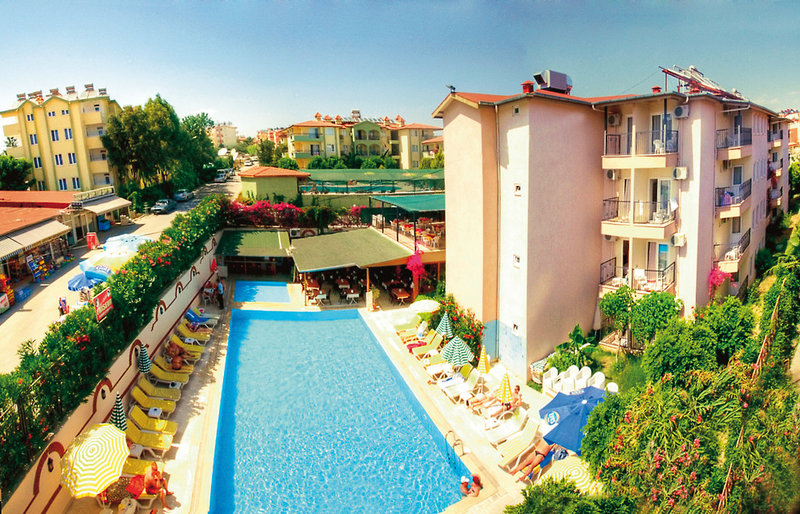
\includegraphics[width=\linewidth]{graphics/kop/aa01.png}
	\caption{Fotografie 1}\label{fig:img01}
	\endminipage\hfill
	\minipage{0.32\textwidth}
	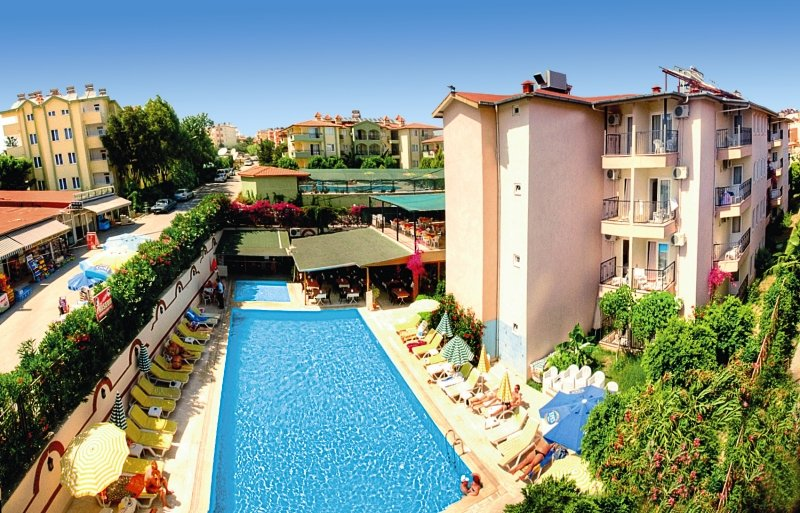
\includegraphics[width=\linewidth]{graphics/kop/aa02.png}
	\caption{Fotografie 2}\label{fig:img02}
	\endminipage\hfill
	\minipage{0.32\textwidth}%
	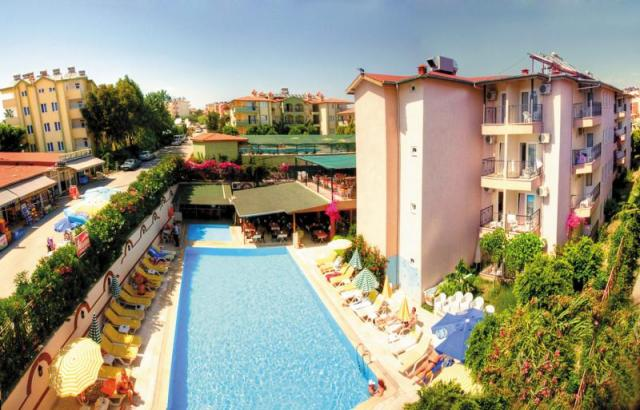
\includegraphics[width=\linewidth]{graphics/kop/aa03.png}
	\caption{Fotografie 3}\label{fig:img03}
	\endminipage\hfill
%\end{figure}
%\begin{figure}[!htb]
	\minipage{0.32\textwidth}%
	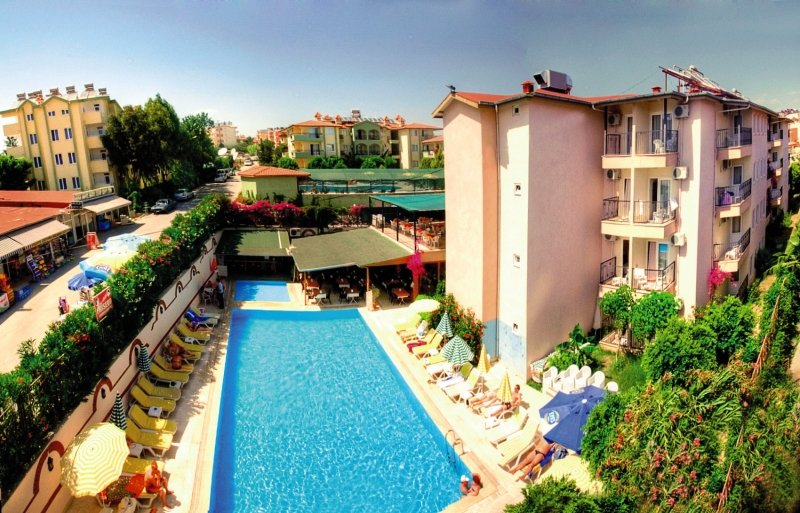
\includegraphics[width=\linewidth]{graphics/kop/aa04.png}
	\caption{Fotografie 4}\label{fig:img04}
	\endminipage\hfill
	\minipage{0.32\textwidth}%
	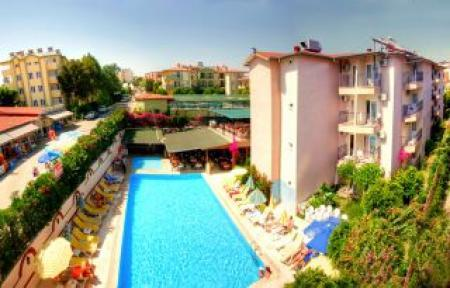
\includegraphics[width=\linewidth]{graphics/kop/aa05.png}
	\caption{Fotografie 5}\label{fig:img05}
	\endminipage\hfill
	\minipage{0.32\textwidth}%
	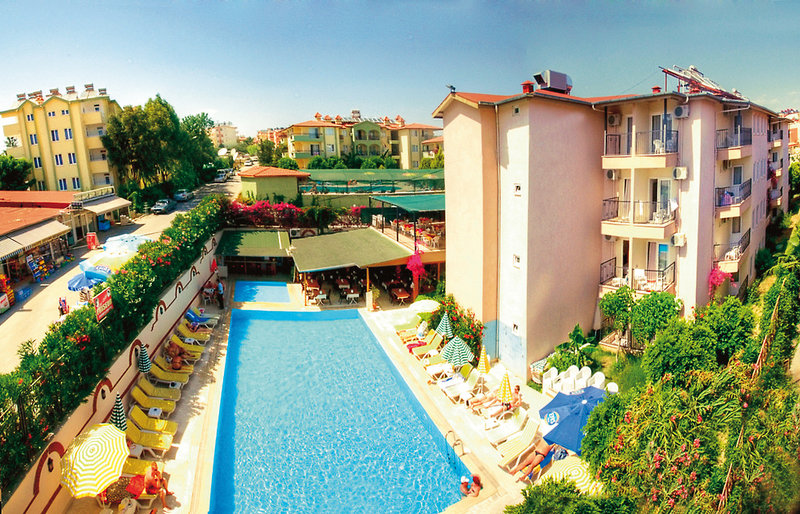
\includegraphics[width=\linewidth]{graphics/kop/aa06.png}
	\caption{Fotografie 6}\label{fig:img06}
	\endminipage\hfill
%\end{figure}
%\begin{figure}[!htb]
	\minipage{0.32\textwidth}%
	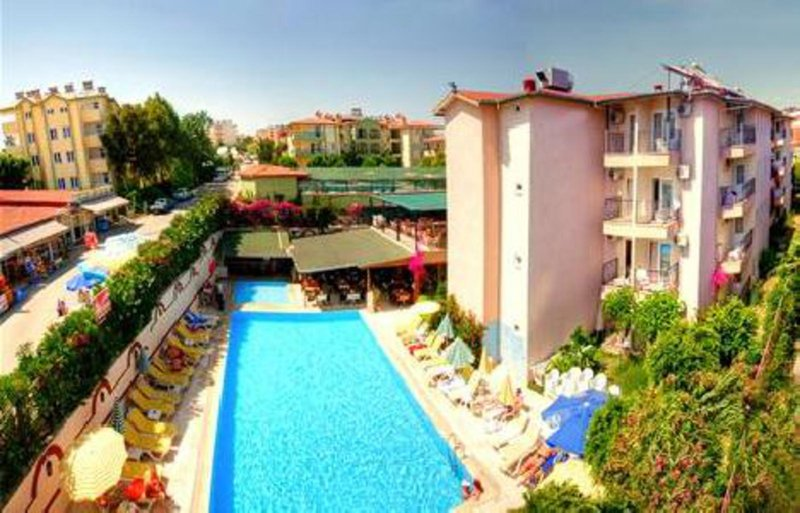
\includegraphics[width=\linewidth]{graphics/kop/aa07.png}
	\caption{Fotografie 7}\label{fig:img07}
	\endminipage\hfill
	\minipage{0.32\textwidth}%
	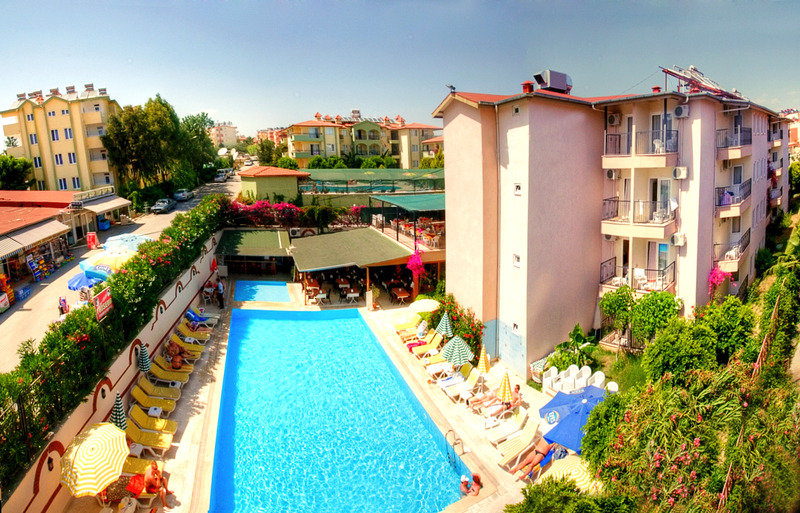
\includegraphics[width=\linewidth]{graphics/kop/aa08.png}
	\caption{Fotografie 8}\label{fig:img08}
	\endminipage\hfill
\end{figure}

Pro~první nalezenou skupinu obsahově duplicitních fotografií byl porovnán koeficient zastupitelnosti KoZ (Tab.~\ref{tab:koz-result}) a~vybrána referenční fotografie (Obr.~\ref{fig:best-photo}) nadále zastupující tuto skupinu. Pro~srovnání je přiložena také fotografie s~nejhorším koeficientem zastupitelnosti ve~skupině (Obr.~\ref{fig:worst-photo}).

\tab {Výsledky porovnání KoZ na 8 podobncýh fotografiích dle KoP} {tab:koz-result} {1.0}
{|r|r|r|r|}
{\hline
							&	Sharpens	&	OverSharpness	&	KoZ				\\	\hline
	\textbf{Fotografie 1}	&	8922		&	432				&	\textbf{35,69}	\\	\hline
	Fotografie 2			&	13228		&	662				&	32,11			\\	\hline
	Fotografie 3			&	1431		&	1				&	5,72			\\	\hline
	Fotografie 4			&	5963		&	115				&	23,85			\\	\hline
	Fotografie 5			&	412			&	0				&	1,65			\\	\hline
	Fotografie 6			&	10900		&	748				&	21,89			\\	\hline
	\textbf{Fotografie 7}	&	261			&	0				&	\textbf{1,04}	\\	\hline
	Fotografie 8			&	8586		&	437				&	34,34			\\	\hline}

\obr{Fotografie s nejvyšším KoZ (nejkvalitnější)}{fig:best-photo}{1.0}{graphics/koz/best-aa01.png}

\obr{Fotografie s nejnižším KoZ (nejméně kvalitní)}{fig:worst-photo}{1.0}{graphics/koz/worst-aa07.png}



% ============================================================================ % % Hlavni text prace

\OdsazovaniOdstavcuStop


% ============================================================================ %
\seznamlit{

  \bibitem{ThinkingInJava}ECKEL, Bruce. \textit{Thinking in Java.} 4th ed. Upper Saddle River, NJ: Prentice Hall, c2006. ISBN 01-318-7248-6.
  
  \bibitem{SpringInAction}WALLS, Craig. \textit{Spring in action.} Fourth edition. Texas: Manning, 2013. ISBN 978-161-7291-203.
  
  \bibitem{JavaPerformance}HUNT, Charlie a Binu JOHN. \textit{Java performance.} Upper Saddle River, NJ: Addison-Wesley, c2012. Java series. ISBN 01-371-4252-8.
  
  \bibitem{matlab}PERŮTKA, Karel. \textit{MATLAB - Základy pro studenty automatizace a informačních technologií.} Zlín: Univerzita Tomáše Bati ve Zlíně, 2005. ISBN 80-731-8355-2.
  
  \bibitem{ImageProcessing}DOBEŠ, Michal. \textit{Zpracování obrazu a algoritmy v C\#.} Praha: BEN - technická literatura, 2008. ISBN 978-80-7300-233-6.

  \bibitem{md5}MD5. In: \it{Wikipedia: the free encyclopedia} [online]. San Francisco (CA): Wikimedia Foundation, 2001- [cit. 2018-05-08]. Dostupné z:~\url{https://en.wikipedia.org/wiki/MD5}.
  
  \bibitem{brightness-matrix}\it{Computer vision} [online]. [cit. 2018-05-08]. Dostupný z:~\url{http://midas.uamt.feec.vutbr.cz/ZVS/Exercise02/content_cz.php}.
  
  \bibitem{pixel}Pixel. \textit{In: Wikipedia: the free encyclopedia} [online]. San Francisco (CA): Wikimedia Foundation, 2001- [cit. 2018-05-08]. Dostupné z:~\url{https://cs.wikipedia.org/wiki/Pixel}.
  
  \bibitem{rgb}RGB. In: \textit{Wikipedia: the free encyclopedia} [online]. San Francisco (CA): Wikimedia Foundation, 2001- [cit. 2018-05-08]. Dostupné z:~\url{https://cs.wikipedia.org/wiki/RGB}.
  
  \bibitem{FFT} \author{BARNEA, Daniel I. a Harvey F. SILVERMAN.} \title{A Class of Algorithms for Fast Digital Image Registration.} \it{IEEE Transactions on Computers} [online]. 1972, \textbf{C-21}(2), 179--186 [cit. 2018-05-08]. DOI: 10.1109/TC.1972.5008923. ISSN 0018-9340. Dostupné z:~\url{http://ieeexplore.ieee.org/document/5008923/}.
  
  \bibitem{correlation}Korelace. In: \textit{Wikipedia: the free encyclopedia} [online]. San Francisco (CA): Wikimedia Foundation, 2001- [cit. 2018-05-09]. Dostupné z:~\url{https://cs.wikipedia.org/wiki/Korelace}.
  
  \bibitem{cross-correlation}Cross-correlation. In: \textit{Wikipedia: the free encyclopedia} [online]. San Francisco (CA): Wikimedia Foundation, 2001- [cit. 2018-05-09]. Dostupné z:~\url{https://en.wikipedia.org/wiki/Cross-correlation}.
  
  \bibitem{fftw}\it{FFTW} [online]. [cit. 2018-05-08]. Dostupný z: \url{http://www.fftw.org}.
  
  \bibitem{fftw3} \author{FRIGO, M. a S.G. JOHNSON.} The Design and Implementation of FFTW3. In: \it{Proceedings of the IEEE} [online]. 2005, \textbf{93}(2), s. 216--231 [cit. 2018-05-08]. DOI: 10.1109/JPROC.2004.840301. ISSN 0018-9219. Dostupné z:~\url{http://ieeexplore.ieee.org/document/1386650}.
  
  \bibitem{FFT-technique} \author{REDDY, B.S. a B.N. CHATTERJI.} \title{An FFT-based technique for translation, rotation, and scale-invariant image registration.} \textit{IEEE Transactions on Image Processing} [online]. \textbf{5}(8), 1266-1271 [cit. 2018-05-08]. DOI: 10.1109/83.506761. ISSN 10577149. Dostupné z:~\url{http://ieeexplore.ieee.org/document/506761/}.
  
  \bibitem{FFT-java}\textit{Shared Scientific Toolbox in Java} [online]. [cit. 2018-05-08]. Dostupné z:~\url{http://freshmeat.sourceforge.net/projects/shared}.
    
  \bibitem{cmake}\it{CMake} [online]. [cit. 2018-05-08]. Dostupný z:~\url{https://cmake.org}.
  
  \bibitem{wrapper}Wrapper. In: \textit{Wikipedia: the free encyclopedia} [online]. San Francisco (CA): Wikimedia Foundation, 2001- [cit. 2018-05-09]. Dostupné z:~\url{https://en.wikipedia.org/wiki/Wrapper}.
  
  \bibitem{convolition}In: \textit{Wikipedia: the free encyclopedia} [online]. San Francisco (CA): Wikimedia Foundation, 2001- [cit. 2018-05-10]. Dostupné z:~\url{https://cs.wikipedia.org/wiki/Konvoluce}.
  
  \bibitem{edge-detection}Detekce hran. In: \textit{Wikipedia: the free encyclopedia} [online]. San Francisco (CA): Wikimedia Foundation, 2001- [cit. 2018-05-10]. Dostupné z:~\url{https://cs.wikipedia.org/wiki/Detekce_hran}.
  
  \bibitem{soap}SOAP. In: \textit{Wikipedia: the free encyclopedia} [online]. San Francisco (CA): Wikimedia Foundation, 2001- [cit. 2018-05-10]. Dostupné z:~\url{https://en.wikipedia.org/wiki/SOAP}.
  
  \bibitem{cpu}Centrální procesorová jednotka. In: \textit{Wikipedia: the free encyclopedia} [online]. San Francisco (CA): Wikimedia Foundation, 2001- [cit. 2018-05-10]. Dostupné z:~\url{https://cs.wikipedia.org/wiki/Centr\%C3\%A1ln\%C3\%AD_procesorov\%C3\%A1_jednotka}.
  
  \bibitem{gpu}Graphic processing unit. In: \textit{Wikipedia: the free encyclopedia} [online]. San Francisco (CA): Wikimedia Foundation, 2001- [cit. 2018-05-10]. Dostupné z:~\url{https://en.wikipedia.org/wiki/Graphics_processing_unit}.
  
  \bibitem{java}Java (programovací jazyk). In: \textit{Wikipedia: the free encyclopedia} [online]. San Francisco (CA): Wikimedia Foundation, 2001- [cit. 2018-05-10]. Dostupné z:~\url{https://cs.wikipedia.org/wiki/Java_(programovac\%C3\%AD_jazyk)}.
  
  \bibitem{cuda}\textit{CUDA Toolkit Documentation} [online]. March 5, 2018 [cit. 2018-05-16]. Dostupné z: \url{https://docs.nvidia.com/cuda/}.
  
  \bibitem{java-se}Java Platform, Standard Edition. In: \textit{Wikipedia: the free encyclopedia} [online]. San Francisco (CA): Wikimedia Foundation, 2001- [cit. 2018-05-16]. Dostupné z:~\url{https://en.wikipedia.org/wiki/Java_Platform,_Standard_Edition}.
  
  \bibitem{spring}\textit{Spring} [online]. 2018 [cit. 2018-05-16]. Dostupné z:~\url{https://spring.io/}.
  
  \bibitem{wsdl}Web Services Description Language. In: \textit{Wikipedia: the free encyclopedia} [online]. San Francisco (CA): Wikimedia Foundation, 2001- [cit. 2018-05-16]. Dostupné z:~\url{https://en.wikipedia.org/wiki/Web_Services_Description_Language}.
  
  \bibitem{postresql}\textit{POSTGRESQL: THE WORLD'S MOST ADVANCED OPEN SOURCE RELATIONAL DATABASE} [online]. The PostgreSQL Global Development Group, 2018 [cit. 2018-05-16]. Dostupné z:~\url{https://www.postgresql.org/}.
  
  \bibitem{challenge-response}Challenge-response. In: \textit{Wikipedia: the free encyclopedia} [online]. San Francisco (CA): Wikimedia Foundation, 2001- [cit. 2018-05-16]. Dostupné z:~\url{https://cs.wikipedia.org/wiki/Challenge-response}.
  
  \bibitem{session}Session. In: \textit{Wikipedia: the free encyclopedia} [online]. San Francisco (CA): Wikimedia Foundation, 2001- [cit. 2018-05-16]. Dostupné z:~\url{https://cs.wikipedia.org/wiki/Session}
  
  \bibitem{hash}Sůl (kryptografie). In:\textit{ Wikipedia: the free encyclopedia} [online]. San Francisco (CA): Wikimedia Foundation, 2001- [cit. 2018-05-16]. Dostupné z:~\url{https://cs.wikipedia.org/wiki/S\%C5\%AFl_(kryptografie)}
  
}

% Pro generování literatury lze alternativně použít i příkaz "\seznamlitbib", 
% který se postará o plnohodnotné vkládání referencí pomocí "bibliography". 
% V takovém případě se využívají bibliografické údaje uložené v souboru 
% tex-literatura.bib. Ty se automaticky upravuji dle zvolené citační normy 
% (v šabloně je nastavena korektní česká norma).
%\seznamlitbib


% ============================================================================ %
% ============================================================================ %
% Encoding: UTF-8 (žluťoučký kůň úpěl ďábelšké ódy)
% ============================================================================ %

\seznamzkr

\begin{tabular}{ll}
  KoP	& Koeficient podobnosti dvou fotografií								\\
  MD5	& Message-Digest algorithm											\\
  px	& picture element (obrazový prvek)									\\
  DFT	& Discrete Fourier Transform (Diskrétní Fourierova transformace)	\\
  IFT	& Inverse Fourier Transform (Zpětná Fourierova transformace)	\\
  FFTW	& Fastest Fourier Transform in the West \\
  ddddd	& test
\end{tabular}

% ============================================================================ %
 % Seznam zkratek


% ============================================================================ %
\seznamobr  % Seznam je generován automaticky


% ============================================================================ %
\seznamtab  % Seznam je generován automaticky


% ============================================================================ %
\seznamscript  % Seznam je generován automaticky


% ============================================================================ %
% ============================================================================ %
% Encoding: UTF-8 (žluťoučký kůň úpěl ďábelšké ódy)
% ============================================================================ %

\listofappendices

\priloha{CD s~průvodními materiály}
Na~CD naleznete
\begin{itemize}
	\item {kompletní zdrojové kódy knihovny pro~výpočet KoP i~KoZ}
	\item {veškerá testovací data (především fotografie)}
	\item {pomocné projekty (např. analýza v~Enterprice Architect)}
\end{itemize}



% ============================================================================ %
 % Prilohy


% ============================================================================ %

\end{document}

% ============================================================================ %
